%%%%%%%%%%%%%%%%%%%%%%%%%%%%%%%%%%%%%%%%%%%%%%%%%%%%%%%%%%%%%%%%%%%%%%
% Template for a UBC-compliant dissertation
% At the minimum, you will need to change the information found
% after the "Document meta-data"
%
%!TEX TS-program = pdflatex
%!TEX encoding = UTF-8 Unicode

%% The ubcdiss class provides several options:
%%   gpscopy (aka fogscopy)
%%       set parameters to exactly how GPS specifies
%%         * single-sided
%%         * page-numbering starts from title page
%%         * the lists of figures and tables have each entry prefixed
%%           with 'Figure' or 'Table'
%%       This can be tested by `\ifgpscopy ... \else ... \fi'
%%   10pt, 11pt, 12pt
%%       set default font size
%%   oneside, twoside
%%       whether to format for single-sided or double-sided printing
%%   balanced
%%       when double-sided, ensure page content is centred
%%       rather than slightly offset (the default)
%%   singlespacing, onehalfspacing, doublespacing
%%       set default inter-line text spacing; the ubcdiss class
%%       provides \textspacing to revert to this configured spacing
%%   draft
%%       disable more intensive processing, such as including
%%       graphics, etc.
%%

% For submission to GPS
\documentclass[gpscopy,onehalfspacing,11pt]{ubcdiss}

% For your own copies (looks nicer)
% \documentclass[balanced,twoside,11pt]{ubcdiss}

%%%%%%%%%%%%%%%%%%%%%%%%%%%%%%%%%%%%%%%%%%%%%%%%%%%%%%%%%%%%%%%%%%%%%%
%%%%%%%%%%%%%%%%%%%%%%%%%%%%%%%%%%%%%%%%%%%%%%%%%%%%%%%%%%%%%%%%%%%%%%
%%
%% FONTS:
%% 
%% The defaults below configures Times Roman for the serif font,
%% Helvetica for the sans serif font, and Courier for the
%% typewriter-style font.  Configuring fonts can be time
%% consuming; we recommend skipping to END FONTS!
%% 
%% If you're feeling brave, have lots of time, and wish to use one
%% your platform's native fonts, see the commented out bits below for
%% XeTeX/XeLaTeX.  This is not for the faint at heart. 
%% (And shouldn't you be writing? :-)
%%

%% NFSS font specification (New Font Selection Scheme)
\usepackage{times,mathptmx,courier}
\usepackage[scaled=.92]{helvet}

%% Math or theory people may want to include the handy AMS macros
\usepackage{amssymb}
\usepackage{amsmath}
%\usepackage{amsfonts}


%% The pifont package provides access to the elements in the dingbat font.   
%% Use \ding{##} for a particular dingbat (see p7 of psnfss2e.pdf)
%%   Useful:
%%     51,52 different forms of a checkmark
%%     54,55,56 different forms of a cross (saltyre)
%%     172-181 are 1-10 in open circle (serif)
%%     182-191 are 1-10 black circle (serif)
%%     192-201 are 1-10 in open circle (sans serif)
%%     202-211 are 1-10 in black circle (sans serif)
%% \begin{dinglist}{##}\item... or dingautolist (which auto-increments)
%% to create a bullet list with the provided character.
\usepackage{pifont}

%%%%%%%%%%%%%%%%%%%%%%%%%%%%%%%%%%%%%%%%%%%%%%%%%%%%%%%%%%%%%%%%%%%%%%
%% Configure fonts for XeTeX / XeLaTeX using the fontspec package.
%% Be sure to check out the fontspec documentation.
%\usepackage{fontspec,xltxtra,xunicode}	% required
%\defaultfontfeatures{Mapping=tex-text}	% recommended
%% Minion Pro and Myriad Pro are shipped with some versions of
%% Adobe Reader.  Adobe representatives have commented that these
%% fonts can be used outside of Adobe Reader.
%\setromanfont[Numbers=OldStyle]{Minion Pro}
%\setsansfont[Numbers=OldStyle,Scale=MatchLowercase]{Myriad Pro}
%\setmonofont[Scale=MatchLowercase]{Andale Mono}

%% Other alternatives:
%\setromanfont[Mapping=tex-text]{Adobe Caslon}
%\setsansfont[Scale=MatchLowercase]{Gill Sans}
%\setsansfont[Scale=MatchLowercase,Mapping=tex-text]{Futura}
%\setmonofont[Scale=MatchLowercase]{Andale Mono}
%\newfontfamily{\SYM}[Scale=0.9]{Zapf Dingbats}
%% END FONTS
%%%%%%%%%%%%%%%%%%%%%%%%%%%%%%%%%%%%%%%%%%%%%%%%%%%%%%%%%%%%%%%%%%%%%%
%%%%%%%%%%%%%%%%%%%%%%%%%%%%%%%%%%%%%%%%%%%%%%%%%%%%%%%%%%%%%%%%%%%%%%



%%%%%%%%%%%%%%%%%%%%%%%%%%%%%%%%%%%%%%%%%%%%%%%%%%%%%%%%%%%%%%%%%%%%%%
%%%%%%%%%%%%%%%%%%%%%%%%%%%%%%%%%%%%%%%%%%%%%%%%%%%%%%%%%%%%%%%%%%%%%%
%%
%% Recommended packages
%%
\usepackage{checkend}	% better error messages on left-open environments
\usepackage{graphicx}	% for incorporating external images

\usepackage{dcolumn}% Align table columns on decimal point.
\usepackage{bm}% bold math.
\usepackage{enumitem}

%% booktabs: provides some special commands for typesetting tables as used
%% in excellent journals.  Ignore the examples in the Lamport book!
\usepackage{booktabs}

%% listings: useful support for including source code listings, with
%% optional special keyword formatting.  The \lstset{} causes
%% the text to be typeset in a smaller sans serif font, with
%% proportional spacing.
\usepackage{listings}
\lstset{basicstyle=\sffamily\scriptsize,showstringspaces=false,fontadjust}

%% The acronym package provides support for defining acronyms, providing
%% their expansion when first used, and building glossaries.  See the
%% example in glossary.tex and the example usage throughout the example
%% document.
%% NOTE: to use \MakeTextLowercase in the \acsfont command below,
%%   we *must* use the `nohyperlinks' option -- it causes errors with
%%   hyperref otherwise.  See Section 5.2 in the ``LaTeX 2e for Class
%%   and Package Writers Guide'' (clsguide.pdf) for details.
\usepackage[printonlyused,nohyperlinks]{acronym}
%% The ubcdiss.cls loads the `textcase' package which provides commands
%% for upper-casing and lower-casing text.  The following causes
%% the acronym package to typeset acronyms in small-caps
%% as recommended by Bringhurst.
\renewcommand{\acsfont}[1]{{\scshape \MakeTextLowercase{#1}}}

%% color: add support for expressing colour models.  Grey can be used
%% to great effect to emphasize other parts of a graphic or text.
%% For an excellent set of examples, see Tufte's "Visual Display of
%% Quantitative Information" or "Envisioning Information".
\usepackage{color}
\definecolor{greytext}{gray}{0.5}

%% comment: provides a new {comment} environment: all text inside the
%% environment is ignored.
%%   \begin{comment} ignored text ... \end{comment}
\usepackage{comment}

%% The natbib package provides more sophisticated citing commands
%% such as \citeauthor{} to provide the author names of a work,
%% \citet{} to produce an author-and-reference citation,
%% \citep{} to produce a parenthetical citation.
%% We use \citeeg{} to provide examples
\usepackage[numbers,sort&compress]{natbib}
\newcommand{\citeeg}[1]{\citep[e.g.,][]{#1}}

%% The titlesec package provides commands to vary how chapter and
%% section titles are typeset.  The following uses more compact
%% spacings above and below the title.  The titleformat that follow
%% ensure chapter/section titles are set in singlespace.
\usepackage[compact]{titlesec}
\titleformat*{\section}{\singlespacing\raggedright\bfseries\Large}
\titleformat*{\subsection}{\singlespacing\raggedright\bfseries\large}
\titleformat*{\subsubsection}{\singlespacing\raggedright\bfseries}
\titleformat*{\paragraph}{\singlespacing\raggedright\itshape}

%% The caption package provides support for varying how table and
%% figure captions are typeset.
\usepackage[format=hang,indention=-1cm,labelfont={bf},margin=1em]{caption}

%% url: for typesetting URLs and smart(er) hyphenation.
%% \url{http://...} 
\usepackage{url}
\urlstyle{sf}	% typeset urls in sans-serif


%%%%%%%%%%%%%%%%%%%%%%%%%%%%%%%%%%%%%%%%%%%%%%%%%%%%%%%%%%%%%%%%%%%%%%
%%%%%%%%%%%%%%%%%%%%%%%%%%%%%%%%%%%%%%%%%%%%%%%%%%%%%%%%%%%%%%%%%%%%%%
%%
%% Possibly useful packages: you may need to explicitly install
%% these from CTAN if they aren't part of your distribution;
%% teTeX seems to ship with a smaller base than MikTeX and MacTeX.
%%
%\usepackage{pdfpages}	% insert pages from other PDF files
%\usepackage{longtable}	% provide tables spanning multiple pages
%\usepackage{chngpage}	% support changing the page widths on demand
%\usepackage{tabularx}	% an enhanced tabular environment

%% enumitem: support pausing and resuming enumerate environments.
%\usepackage{enumitem}

%% rotating: provides two environments, sidewaystable and sidewaysfigure,
%% for typesetting tables and figures in landscape mode.  
\usepackage{rotating}
\usepackage{pdflscape}

%% subfig: provides for including subfigures within a figure,
%% and includes being able to separately reference the subfigures.
\usepackage{subfig}

%% ragged2e: provides several new new commands \Centering, \RaggedLeft,
%% \RaggedRight and \justifying and new environments Center, FlushLeft,
%% FlushRight and justify, which set ragged text and are easily
%% configurable to allow hyphenation.
%\usepackage{ragged2e}

%% The ulem package provides a \sout{} for striking out text and
%% \xout for crossing out text.  The normalem and normalbf are
%% necessary as the package messes with the emphasis and bold fonts
%% otherwise.
%\usepackage[normalem,normalbf]{ulem}    % for \sout

%%%%%%%%%%%%%%%%%%%%%%%%%%%%%%%%%%%%%%%%%%%%%%%%%%%%%%%%%%%%%%%%%%%%%%
%% HYPERREF:
%% The hyperref package provides for embedding hyperlinks into your
%% document.  By default the table of contents, references, citations,
%% and footnotes are hyperlinked.
%%
%% Hyperref provides a very handy command for doing cross-references:
%% \autoref{}.  This is similar to \ref{} and \pageref{} except that
%% it automagically puts in the *type* of reference.  For example,
%% referencing a figure's label will put the text `Figure 3.4'.
%% And the text will be hyperlinked to the appropriate place in the
%% document.
%%
%% Generally hyperref should appear after most other packages

%% The following puts hyperlinks in very faint grey boxes.
%% The `pagebackref' causes the references in the bibliography to have
%% back-references to the citing page; `backref' puts the citing section
%% number.  See further below for other examples of using hyperref.
%% 2009/12/09: now use `linktocpage' (Jacek Kisynski): GPS now prefers
%%   that the ToC, LoF, LoT place the hyperlink on the page number,
%%   rather than the entry text.
\usepackage[bookmarks,bookmarksnumbered,%
    allbordercolors={0.8 0.8 0.8},%
    pagebackref,linktocpage%
    ]{hyperref}
%% The following change how the the back-references text is typeset in a
%% bibliography when `backref' or `pagebackref' are used
\renewcommand\backrefpagesname{\(\rightarrow\) pages}
\renewcommand\backref{\textcolor{greytext} \backrefpagesname\ }

%% The following uses most defaults, which causes hyperlinks to be
%% surrounded by colourful boxes; the colours are only visible in
%% PDFs and don't show up when printed:
%\usepackage[bookmarks,bookmarksnumbered]{hyperref}

%% The following disables the colourful boxes around hyperlinks.
%\usepackage[bookmarks,bookmarksnumbered,pdfborder={0 0 0}]{hyperref}

%% The following disables all hyperlinking, but still enabled use of
%% \autoref{}
%\usepackage[draft]{hyperref}

%% The following commands causes chapter and section references to
%% uppercase the part name.
\renewcommand{\chapterautorefname}{Chapter}
\renewcommand{\sectionautorefname}{Section}
\renewcommand{\subsectionautorefname}{Section}
\renewcommand{\subsubsectionautorefname}{Section}

%% If you have long page numbers (e.g., roman numbers in the 
%% preliminary pages for page 28 = xxviii), you might need to
%% uncomment the following and tweak the \@pnumwidth length
%% (default: 1.55em).  See the tocloft documentation at
%% http://www.ctan.org/tex-archive/macros/latex/contrib/tocloft/
% \makeatletter
% \renewcommand{\@pnumwidth}{3em}
% \makeatother

%%%%%%%%%%%%%%%%%%%%%%%%%%%%%%%%%%%%%%%%%%%%%%%%%%%%%%%%%%%%%%%%%%%%%%
%%%%%%%%%%%%%%%%%%%%%%%%%%%%%%%%%%%%%%%%%%%%%%%%%%%%%%%%%%%%%%%%%%%%%%
%%
%% Some special settings that controls how text is typeset
%%
% \raggedbottom		% pages don't have to line up nicely on the last line
% \sloppy		% be a bit more relaxed in inter-word spacing
% \clubpenalty=10000	% try harder to avoid orphans
% \widowpenalty=10000	% try harder to avoid widows
% \tolerance=1000

%% And include some of our own useful macros
% This file provides examples of some useful macros for typesetting
% dissertations.  None of the macros defined here are necessary beyond
% for the template documentation, so feel free to change, remove, and add
% your own definitions.
%
% We recommend that you define macros to separate the semantics
% of the things you write from how they are presented.  For example,
% you'll see definitions below for a macro \file{}: by using
% \file{} consistently in the text, we can change how filenames
% are typeset simply by changing the definition of \file{} in
% this file.
% 
%% The following is a directive for TeXShop to indicate the main file
%%!TEX root = diss.tex

\newcommand{\NA}{\textsc{n/a}}	% for "not applicable"
\newcommand{\eg}{e.g.,\ }	% proper form of examples (\eg a, b, c)
\newcommand{\ie}{i.e.,\ }	% proper form for that is (\ie a, b, c)
\newcommand{\etal}{\emph{et al}}

% Some useful macros for typesetting terms.
\newcommand{\file}[1]{\texttt{#1}}
\newcommand{\class}[1]{\texttt{#1}}
\newcommand{\latexpackage}[1]{\href{http://www.ctan.org/macros/latex/contrib/#1}{\texttt{#1}}}
\newcommand{\latexmiscpackage}[1]{\href{http://www.ctan.org/macros/latex/contrib/misc/#1.sty}{\texttt{#1}}}
\newcommand{\env}[1]{\texttt{#1}}
\newcommand{\BibTeX}{Bib\TeX}

% Define a command \doi{} to typeset a digital object identifier (DOI).
% Note: if the following definition raise an error, then you likely
% have an ancient version of url.sty.  Either find a more recent version
% (3.1 or later work fine) and simply copy it into this directory,  or
% comment out the following two lines and uncomment the third.
\DeclareUrlCommand\DOI{}
\newcommand{\doi}[1]{\href{http://dx.doi.org/#1}{\DOI{doi:#1}}}
%\newcommand{\doi}[1]{\href{http://dx.doi.org/#1}{doi:#1}}

% Useful macro to reference an online document with a hyperlink
% as well with the URL explicitly listed in a footnote
% #1: the URL
% #2: the anchoring text
\newcommand{\webref}[2]{\href{#1}{#2}\footnote{\url{#1}}}

% epigraph is a nice environment for typesetting quotations
\makeatletter
\newenvironment{epigraph}{%
	\begin{flushright}
	\begin{minipage}{\columnwidth-0.75in}
	\begin{flushright}
	\@ifundefined{singlespacing}{}{\singlespacing}%
    }{
	\end{flushright}
	\end{minipage}
	\end{flushright}}
\makeatother

% \FIXME{} is a useful macro for noting things needing to be changed.
% The following definition will also output a warning to the console
\newcommand{\FIXME}[1]{\typeout{**FIXME** #1}\textbf{[FIXME: #1]}}

% END


%%%%%%%%%%%%%%%%%%%%%%%%%%%%%%%%%%%%%%%%%%%%%%%%%%%%%%%%%%%%%%%%%%%%%%
%%%%%%%%%%%%%%%%%%%%%%%%%%%%%%%%%%%%%%%%%%%%%%%%%%%%%%%%%%%%%%%%%%%%%%
%%
%% Document meta-data: be sure to also change the \hypersetup information
%%

\title{Simulations of an Areogel Ring Imaging Cherenkov Detector for Particle Identification}
%\subtitle{If you want a subtitle}

\author{Daniel Levy}

% What is this dissertation for?
\degreetitle{Bachelor of Science}

\institution{The University of British Columbia}
\campus{Vancouver}

\faculty{The Faculty of Science}
\department{Department of Physics and Astronomy}
\submissionmonth{April}
\submissionyear{2019}

%% hyperref package provides support for embedding meta-data in .PDF
%% files
\hypersetup{
  pdftitle={Change this title!  (DRAFT: \today)},
  pdfauthor={Johnny Canuck},
  pdfkeywords={Your keywords here}
}

%%%%%%%%%%%%%%%%%%%%%%%%%%%%%%%%%%%%%%%%%%%%%%%%%%%%%%%%%%%%%%%%%%%%%%
%%%%%%%%%%%%%%%%%%%%%%%%%%%%%%%%%%%%%%%%%%%%%%%%%%%%%%%%%%%%%%%%%%%%%%
%% 
%% The document content
%%

%% LaTeX's \includeonly commands causes any uses of \include{} to only
%% include files that are in the list.  This is helpful to produce
%% subsets of your thesis (e.g., for committee members who want to see
%% the dissertation chapter by chapter).  It also saves time by 
%% avoiding reprocessing the entire file.
%\includeonly{intro,conclusions}
%\includeonly{discussion}

\begin{document}

%%%%%%%%%%%%%%%%%%%%%%%%%%%%%%%%%%%%%%%%%%%%%%%%%%
%% From Thesis Components: Tradtional Thesis
%% <http://www.grad.ubc.ca/current-students/dissertation-thesis-preparation/order-components>

% Preliminary Pages (numbered in lower case Roman numerals)
%    1. Title page (mandatory)
\maketitle

%    2. Abstract (mandatory - maximum 350 words)
%% The following is a directive for TeXShop to indicate the main file
%%!TEX root = diss.tex

\chapter{Abstract}

In next-generation accelerator-based neutrino detectors such as Hyper-Kamiokande and DUNE, one of the leading sources of uncertainties lies in the calculations of neutrino flux. The \ac{EMPHATIC} aims to improve calculations of neutrino flux by measuring hadron production resulting from a test proton beam hitting a variety of targets. \ac{EMPHATIC} includes an Aerogel Ring Imaging Cherenkov detector, which uses the distribution of detected photons resulting from Cherenkov radiation in order to determine particle velocity. A Monte Carlo simulation is created of particles travelling through the detector, and the propagation of the generated Cherenkov radiation is simulated. Using a likelihood approach, evaluation of the simulated photon distributions allows for the identification of particles.

% Consider placing version information if you circulate multiple drafts
\vfill
\begin{center}
\begin{sf}
\fbox{Revision: \today}
\end{sf}
\end{center}

\cleardoublepage

%    3. Preface
%%% The following is a directive for TeXShop to indicate the main file
%%!TEX root = diss.tex

\chapter{Preface}

At \ac{UBC}, a preface may be required.  Be sure to check the
\ac{GPS} guidelines as they may have specific content to be included.

%\cleardoublepage

%    4. Table of contents (mandatory - list all items in the preliminary pages
%    starting with the abstract, followed by chapter headings and
%    subheadings, bibliographies and appendices)
\tableofcontents
\cleardoublepage	% required by tocloft package

%    5. List of tables (mandatory if thesis has tables)
% \listoftables
% \cleardoublepage	% required by tocloft package

%    6. List of figures (mandatory if thesis has figures)
\listoffigures
\cleardoublepage	% required by tocloft package

%    7. List of illustrations (mandatory if thesis has illustrations)
%    8. Lists of symbols, abbreviations or other (optional)

%    9. Glossary (optional)
%% The following is a directive for TeXShop to indicate the main file
%%!TEX root = diss.tex

\chapter{Glossary}

This glossary uses the handy \latexpackage{acroynym} package to automatically
maintain the glossary.  It uses the package's \texttt{printonlyused}
option to include only those acronyms explicitly referenced in the
\LaTeX\ source.

% use \acrodef to define an acronym, but no listing
\acrodef{UI}{user interface}
\acrodef{UBC}{University of British Columbia}

% The acronym environment will typeset only those acronyms that were
% *actually used* in the course of the document
\begin{acronym}
\acro{EMPHATIC}{The Experiment Measuring Production of Hadrons at a Test beam in Chicagoland}
\acro{RPC ToF}{Resistive Plate Chamber Time-of-Flight}
\acro{ARICH}{Aerogel Ring Imaging Cherenkov}
\acro{PMT}{Photomultiplier Tube}
\acro{SSD}{Silicon Strip Detector}
\acro{ROOT}{An object-oriented }
\acro{API}{application programming interface}
\acro{CTAN}{\acroextra{The }Common \TeX\ Archive Network}
\acro{DOI}{Document Object Identifier\acroextra{ (see
    \url{http://doi.org})}}
\acro{GPS}[GPS]{Graduate and Postdoctoral Studies}
\acro{PDF}{Portable Document Format}
\acro{RCS}[RCS]{Revision control system\acroextra{, a software
    tool for tracking changes to a set of files}}
\acro{TLX}[TLX]{Task Load Index\acroextra{, an instrument for gauging
  the subjective mental workload experienced by a human in performing
  a task}}
\acro{UML}{Unified Modelling Language\acroextra{, a visual language
    for modelling the structure of software artefacts}}
\acro{URL}{Unique Resource Locator\acroextra{, used to describe a
    means for obtaining some resource on the world wide web}}
\acro{W3C}[W3C]{\acroextra{the }World Wide Web Consortium\acroextra{,
    the standards body for web technologies}}
\acro{XML}{Extensible Markup Language}
\end{acronym}

% You can also use \newacro{}{} to only define acronyms
% but without explictly creating a glossary
% 
% \newacro{ANOVA}[ANOVA]{Analysis of Variance\acroextra{, a set of
%   statistical techniques to identify sources of variability between groups.}}
% \newacro{API}[API]{application programming interface}
% \newacro{GOMS}[GOMS]{Goals, Operators, Methods, and Selection\acroextra{,
%   a framework for usability analysis.}}
% \newacro{TLX}[TLX]{Task Load Index\acroextra{, an instrument for gauging
%   the subjective mental workload experienced by a human in performing
%   a task.}}
% \newacro{UI}[UI]{user interface}
% \newacro{UML}[UML]{Unified Modelling Language}
% \newacro{W3C}[W3C]{World Wide Web Consortium}
% \newacro{XML}[XML]{Extensible Markup Language}
	% always input, since other macros may rely on it

\textspacing		% begin one-half or double spacing

%   10. Acknowledgements (optional)
%% The following is a directive for TeXShop to indicate the main file
%%!TEX root = diss.tex

\chapter{Acknowledgments}
I would like to thank my supervisor, Dr. Mark Hartz, for all his guidance in planning out this thesis project and giving me the fantastic opportunity to work with the neutrino group at TRIUMF.
I would also like to thank Dr. Matej Pavin and Dr. Akira Konaka for their helping me understand the context of \ac{EMPHATIC} and for help with my computational needs.
Lastly I would like to thank Dr. Rob Kiefl for his invaluable help.


%   11. Dedication (optional)

% Body of Thesis (not all sections may apply)
\mainmatter

\acresetall	% reset all acronyms used so far

%    1. Introduction
%% The following is a directive for TeXShop to indicate the main file
%%!TEX root = diss.tex

\chapter{Introduction}
\label{ch:Introduction}

%%%%%%%%%%%%%%%%%%%%%%%%%%%%%%%%%%%%%%%%%%%%%%%%%%%%%%%%%%%%%%%%%%%%%%
\section{Motivation}

Since the neutrino was first postulated by Wolfgang Pauli in 1930 \cite{neutrinoHistory}, neutrinos have proven to be an important probe into various fundamental properties of our universe.
Because neutrinos do not react via the electromagnetic or strong force, they may only be detected via the weak force, presenting a significant challenge to any attempts to measure them.
Over the past 60 years, physicists have built increasingly sophisticated and sensitive detectors to accurately measure the properties of these particles.

There are three flavors of neutrinos: the electron neutrino $\nu_e$, the muon neutrino $\nu_\mu$, and the tau neutrino $\nu_\tau$.
The flavor of the neutrino determines what interactions it might have.
In 1998, the Super-Kamiokande detector in Japan observed clear evidence of neutrino oscillation: as neutrinos of one flavor travels over a large distance, it has some probability of later being observed as a neutrino of another generation.
This implied that neutrinos have a nonzero mass, a result not predicted by the Standard Model.
The theorized explanation for neutrino oscillation is that each neutrino flavor actually exists as some superposition of 3 different mass states. As a neutrino travels over large distances, the differences in phases of the mass states results in a shifting probability of detecting each neutrino flavor.
The relationship between mass and flavor states is governed by the following relation:

\begin{equation}
\begin{pmatrix}
\nu_e \\ \nu_\mu \\ \nu_\tau
\end{pmatrix}
=
%U
\begin{pmatrix}
U_{e1} & U_{e1} & U_{e1} \\ 
U_{\mu 1} & U_{\mu 2} & U_{\mu 3} \\
U_{\tau 1} & U_{\tau 2} & U_{\tau 3}
\end{pmatrix}
\begin{pmatrix}
\nu_1 \\ \nu_2 \\ \nu_3
\end{pmatrix}
\end{equation}

Here, U is a $3 \times 3$ unitary matrix, known as the Pontecorvo–Maki–Nakagawa–Sakata (PMNS) Matrix. The matrix can be characterized by 4 parameters: $\theta_{12}, \theta_{23}$, and $\theta_{13}$, which are the mixing angles, and $\delta_{CP}$, known as the CP-violating phase \cite{pdg2018}. The probability of a neutrino oscillating from one flavor to another is governed by the distance travelled, the mixing angles, and $\Delta m_{ij}^2$, the squared mass difference between neutrino states. 


There are many open-ended questions regarding neutrinos.
The mixing angles of the PMNS matrix and the squared mass differences remain to be more accurately measured.
Because only the differences in masses are known, the actual ordering and absolute values of the masses are unknown.
It is unknown whether neutrinos are their own anti-particles (i.e. whether the neutrino is a Majorana fermion), or if the antineutrino is a distinct particle (i.e. a Dirac fermion).
It is uncertain whether $\sin(\delta_{CP})$ is consistent with zero: If it is nonzero, then that may explain the asymmetry between the amount of matter and antimatter in the universe \cite{neutrinoCP}.

The next generation of neutrino experiments aim to answer all of these questions (and more) to a high degree of precision - they include the Deep Underground Neutrino Experiment (DUNE) \cite{duneDesign} and the Hyper-Kamiokande experiment \cite{hyperKDesign}.
In both experiments, a large flux of neutrinos is generated with a particle accelerator hundreds of kilometers away from a large neutrino detector.
When a sufficiently energetic particle beam hits a target, the collision produces secondary particles: mostly charged pions and kaons.
Magnetic horns are used to direct these secondary particles in the direction of the distant detector. \TODO{introduce the term ``hadron"} 
The charged pions will decay in flight as follows:

\begin{equation}
\pi^+ \rightarrow \mu^+ + \nu_\mu \quad   \text{and} \quad \mu^+ \rightarrow \bar{\nu}_e + \nu_\mu
\end{equation}

The charged kaons have several decay modes, but the most common are:

\begin{equation}
K^+ \rightarrow \mu^+ + \nu_\mu \text{,} \quad  K^+ \rightarrow \pi^+ + \pi^0  \text{,}\quad K^+ \rightarrow \pi^0 + e^+ + \nu_e
\end{equation}

There are corresponding charge-conjugate decays for the $\pi^-$ and $K^-$. 
As these secondary particles decay, a large number of resulting neutrinos are sent in the direction of the detector, where only a very small fraction will be detected.

These next-generation neutrino experiments have a far higher level of statistics than in neutrino experiments of the past, due to the massive size of the detectors.
Because the error is no longer dominated by statistical error, decreasing any systematic error is increasingly important.
In such experiments, the two major sources of systematic error arises from uncertainty in the neutrino-nucleus interaction, and uncertainty in calculations of the neutrino flux.
The primary contribution to the uncertainty of neutrino flux lies in uncertainty in the hadron production \cite{hyperKDesign}.

The NA61/SHINE experiment, located at CERN, has been very successful in measuring hadron production resulting from collisions of particles from the Super Proton Synchrotron onto various targets \cite{na61}.
These measurements significantly reduced neutrino flux uncertainties in T2K, an ongoing accelerator-based neutrino oscillation experiment \cite{na61T2K}. 
However, the momenta of the measured beams are constrained to between 13 and 160 GeV/c.
This does not allow for the calculations of low-momentum hadron reinteractions: in addition to hadrons directly decaying into neutrinos, some hadrons may reinteract with the target, magnetic horns, or beamline of the detector, affecting the neutrino flux.
Furthermore, some neutrino experiments aim to measure atmospheric neutrinos (neutrinos resulting from the decay of products of the reaction of cosmic rays with the atmosphere), and the NA61/SHINE data does not cover the associated lower-momentum hadron interactions.

 \section{\ac{EMPHATIC}}

In order to constrain hadron production uncertainties, work is in progress for EMPHATIC (Experiment Measuring the Production of Hadrons At a Test-beam In Chicagoland).
EMPHATIC is a tabletop experiment designed to precisely measure hadron interactions resulting from a proton or pion beam impinging on various targets. 
EMPHATIC is located at the Fermilab Test Beam Facility, and the proposed experimental setup is shown in Figure \ref{fig:EMPHATIC}.
The Fermilab Test Beam can produce a beam with momenta ranging from 0.2-120 GeV, which complements the momenta measured by NA61/SHINE.

\begin{figure}[] 
\centering
\resizebox{0.75\textwidth}{!}{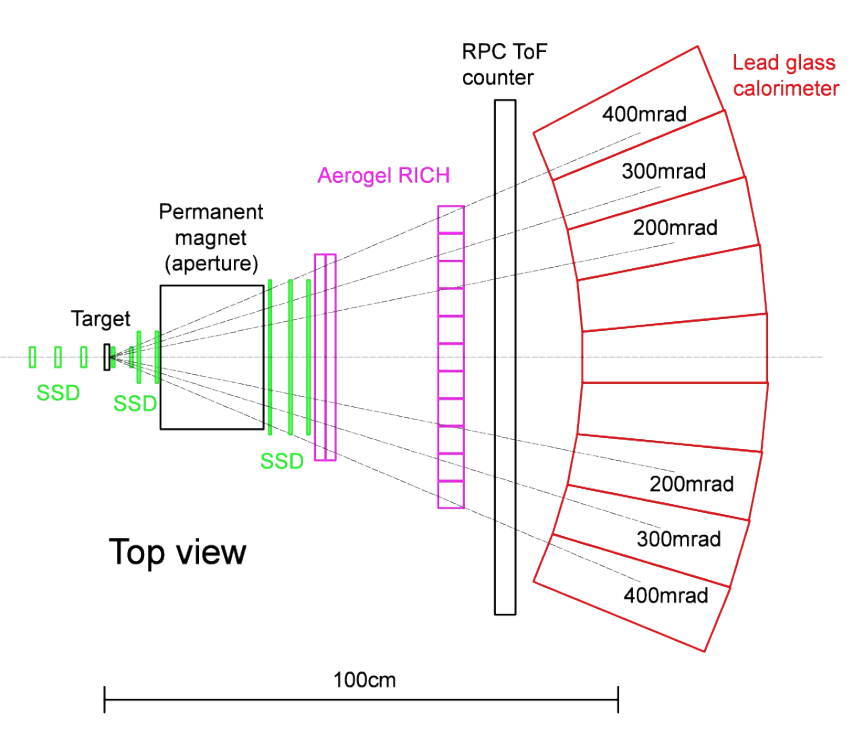
\includegraphics{./figs/EMPHATIC.png}}
\caption[Top view of the proposed EMPHATIC setup]{Top view of the proposed EMPHATIC setup, obtained with permission from the EMPHATIC group. The different detectors in the setup are shown in different colours.}
\label{fig:EMPHATIC} 
\end{figure}

To obtain measurements for accelerator-based neutrino experiments, \ac{EMPHATIC} will measure targets of graphite, aluminum, and iron.
These targets correspond to the composition of the proposed targets, magnetic horns, and beamline components typically found in accelerator-based neutrino experiments.
\ac{EMPHATIC} will also measure targets composed of boron, boron nitride, and boron trioxide.
Because the atmosphere is primarily composed of nitrogen and oxygen, measuring the latter two targets and removing the effects of pure boron will lead to an estimation of hadron production arising from the interaction of cosmic rays in the atmosphere. 

\ac{EMPHATIC} includes four different kinds of detectors that serve to measure hadron production.
A set of silicon strip detectors (SSDs) register the position of each particle as they pass through.
A permanent magnet downstream of the target causes the trajectory of particles to curve due to the Lorentz force: the radius of the curvature is proportional to momentum of the particle.
By using multiple SSDs downstream of the magnet, particle momenta and trajectories may be measured.
The particles then pass through an Aerogel Ring Imaging Cherenkov (ARICH) detector.
As explained in Section \ref{sec:ARICH}, this detector can be used to determine a charged particle's velocity if its trajectory is known. 
If the velocity and momentum of a particle are known, then its mass may be determined.
This allows for the identification of each particle. 

After passing through the ARICH detector, particles will pass through a resistive plate chamber time-of-flight (RPC ToF) detector.
This detector measures the time at which a particle passes through and compares this to an upstream measurement, giving another measure of velocity. 
Unlike the ARICH detector, the ToF detector does not have the resolution sufficient to properly identify forward-angle high-momentum particles, but due to its greater angular coverage, it is able to identify lower-momentum particles.
These two detectors complement each other to provide a full measurement of velocities across a broad range.
Following this, particles strike a lead glass calorimeter, which measures the final particle energy.
The lead glass calorimeter is useful for identifying electrons or neutrons.

\section{Overview of the project}
Development is underway on the simulation and design of the ARICH detector for EMPHATIC.
The ARICH detector should be able to accurately distinguish between charged pions, charged kaons, and protons over a broad spectrum of momenta.
We propose to use the ARICH detector to conduct particle identification by using a likelihood approach. 
With this approach, photon measurements from each experimental event are compared against several different Monte Carlo simulations of that event, each representing a different hypothesis for what particle or particles were involved.
The particle or particles that produced the simulated distribution that best matches the experimental data is then chosen as the most likely candidate.
This technique is fully described in Chapter \ref{sec:particleIdentification}. 

Concurrent work is underway for a full end-to-end Monte Carlo simulation of the EMPHATIC experimental setup.
This simulation is created using Geant4, a platform designed for Monte Carlo simulations of particles passing through matter \cite{geant4}.
This simulation will contain information on the placement of all detector components and their materials, and models the physical interactions of each particle running through the experiment, and the shower of secondary particles produced. \TODO{Awkward sentence}
While the Geant4 simulation should give accurate results for the distribution of optical photons for different particle hypotheses, it is relatively slow to perform a full simulation for each particle.
Using the proposed likelihood approach to particle identification, we would be required to run several different simulations per experimental event.
The Geant4 simulation is therefore too slow to be run as a tool for particle identification, necessitating the need for a more efficient fast simulation of just the optical processes in the ARICH detector. 

In this project, I created such a fast simulation that incorporates the relevant physical processes while maintaining high efficiency.
The simulation is described in Chapter \ref{ch:Methods}.
Following this, the particle identification performance of this technique was evaluated under several different conditions, which are described in Chapter \ref{ch:Results}.

\endinput

Any text after an \endinput is ignored.
You could put scraps here or things in progress.


%    2. Main body
%% The following is a directive for TeXShop to indicate the main file
%%!TEX root = diss.tex

\chapter{Theory}
\label{ch:Theory}

\section{Cherenkov Radiation}
\label{sec:cherenkov}
Although the speed of light in a vacuum is a constant $c$, when light passes through a medium with a refractive index of $n$, it will travel at the velocity $c/n$.
When a charged particle travels through a dielectric medium (known as a radiator) at a velocity greater than the speed of light in the medium, it will displace electrons, emitting photons radially at points along the particle's path.
This process is known as Cherenkov radiation \cite{cherenkov}.
If we define the particle velocity to be $v_p$ and $\beta = v_p / c$, then in a time $t$, the particle will travel a distance $\beta ct$.
In that same amount of time, the photons emitted in the radiator will have travelled a distance $(c/n)t$.
The geometry of this emission is shown in in Figure \ref{fig:cherenkov}.
This creates a wavefront of light emitted obeying the following relation:
\begin{equation}
    cos(\theta) = \frac{1}{\beta n}
    \label{eq:cherenkovAngle}
\end{equation}

\begin{figure}[]
\centering
\resizebox{0.8\textwidth}{!}{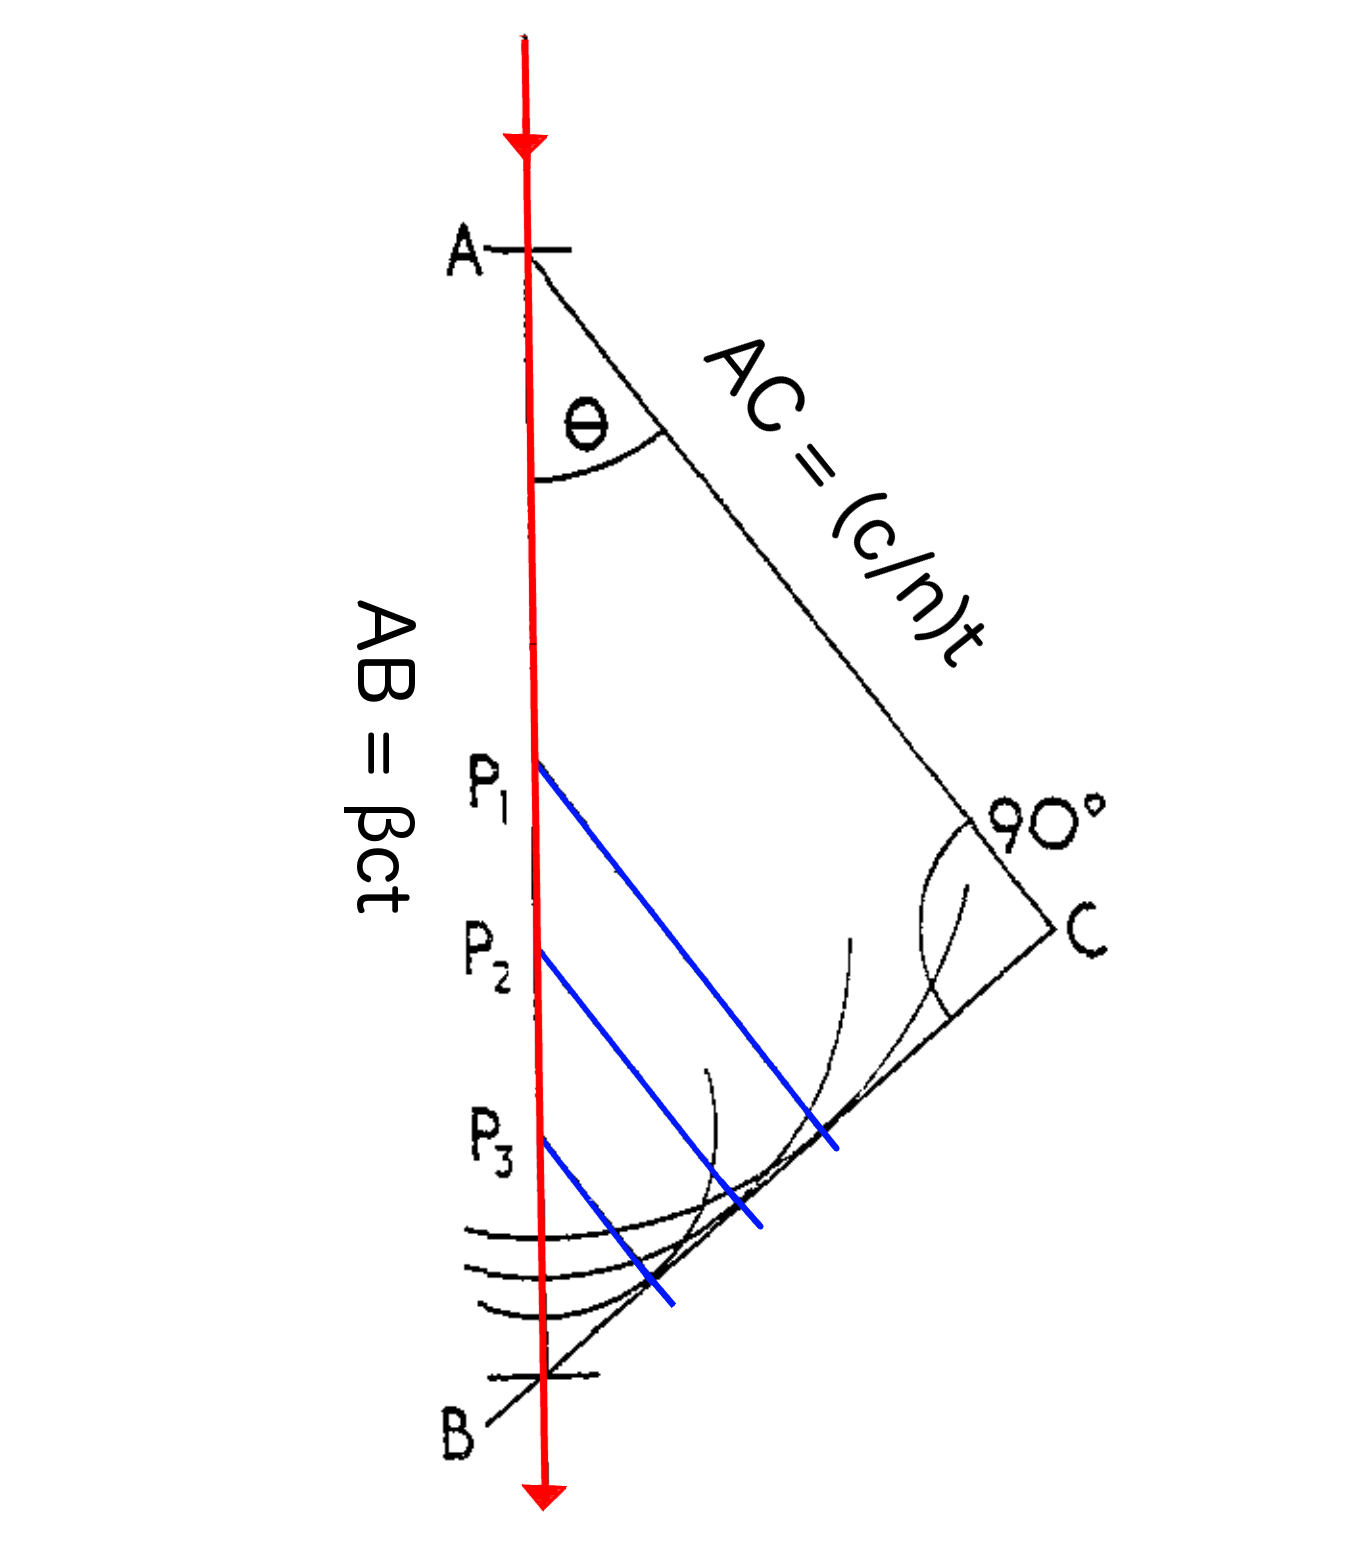
\includegraphics{./figs/cherenkovMod.png}}
\caption[Diagram showing the emission of Cherenkov radiation]{Diagram showing the emission of Cherenkov radiation, adapted from \cite{cherenkov}.
In this diagram, a particle travels along the vertical line from point A to point B.
Electromagnetic radiation is emitted at $P_1$, $P_2$, and $P_3$, each producing one of the curves shown.
It can be seen that these emissions all produce a wavefront along BC, giving a common angle of emission $\theta$.}
\label{fig:cherenkov} 
\end{figure}

The energy emitted via Cherenkov radiation by a particle of charge $q$ as it moves a distance $dl$ through a radiator is given by the Frank-Tamm formula \cite{frankTamm}:
\begin{equation}
    \label{eq:frankTamm}
    \frac{dW}{dl} = \frac{q^2}{c^2}\int_{\beta n > 1} \omega  \left(1 - \frac{1}{\beta^2n(\omega)^2}\right)d\omega
\end{equation}

In this formula, $\omega$ is the angular frequency of the light.
If we neglect the frequency dependence of the index of refraction, then we can use this equation to extract the expected number of photons emitted per length $dl$ over a range of frequencies from $\lambda_1$ to $\lambda_2$:

\begin{equation}
    \label{eq:photonNumber}
    \frac{dN}{dl}  = 2\pi\alpha q^2 \left(\frac{1}{\lambda_2} - \frac{1}{\lambda_1}
    \right)\left(1 - \frac{1}{\beta^2n^2}\right)
\end{equation}

Here, $\alpha$ is the fine structure constant ($\approx \frac{1}{137}$).



\section{Aerogel Ring Imaging Cherenkov Detectors}
\label{sec:ARICH}
The relationship between particle velocity through a radiator and photon angle of emission (Equation \ref{eq:cherenkovAngle}) can be exploited for particle identification.
An \ac{ARICH} detector consists of a silica aerogel radiator, and an array of \ac{PMT}s, which can detect Cherenkov radiation of charged particles passing through the aerogel.
Silica aerogel is a substance made of a network of silica (SiO$_2$) clusters interspersed with nanopores of air \cite{aerogelRefraction}.
During production, the refractive index of aerogel can be precisely tuned \cite{aerogelRefraction}, and the wavelength-dependency of the refractive index is understood \cite{aerogelWavelength}. 



High-velocity charged particles produced in the collision of the hadron beam with a target will emit cones of Cherenkov radiation as they travel through the aerogel, leading to an elliptically shaped set of detected photons.
As the angle of emission depends on the velocity of a particle, the radii of the ellipses depend just on the velocity of the particle, the distance between the point of emission and the detector, and the angle of the incident charged particle.

At the time of this project, the aerogels available for use for EMPHATIC had indices of refraction of 1.035, 1.04, 1.045, and 1.05.
Looking at Equation \ref{eq:cherenkovAngle}, we see that with a lower index of refraction, the Cherenkov angle changes more rapidly with respect to particle velocity. 
A rapidly changing angle would allow for the velocity of a particle to be better resolved, and so the aerogel with an index of refraction of 1.035 was chosen to be used in the detector.

By averaging over several photons emitted by a single particle, we can increase our angular resolution.
With a thicker slab of aerogel, a charged particle travels a greater distance and is likely to emit a greater number of photons.
However, this means that the point of emission of the photon can vary more, reducing the angular resolution.
To combat this, \ac{ARICH} detectors can use two or more layers of aerogel with differing indices of refraction, with the layer closest to the detector having a higher index of refraction \cite{belleArich}.
The photons emitted in the first layer will be emitted at a smaller angle than those from the second layer, and ultimately arrive on the same ring on the photon detector array.
The Cherenkov radius of a photon emitted from a charged particle travelling directly downstream at a velocity $\beta$, through a layer of aerogel with an index of refraction $n$ and a distance $d$ from the detector plane is given by:

\begin{equation}
d\tan\left(\arccos\left(\frac{1}{\beta n}\right)\right)
\end{equation}

For EMPHATIC, the slabs of aerogel were chosen to be 2 cm thick, and the first layer was chosen to be placed with its centre at a distance of 20 cm from the photon detector plane.
If the first layer has an index of refraction of $n = 1.035$, then to most closely match the Cherenkov radius for a typical particle velocity of $\beta \approx 1$, the best available value for the index of refraction of a second layer of aerogel placed 18 cm upstream of the detector plane would be 1.045. 
Since the start of this project, an aerogel with an index of refraction of 1.03 has become available.
However, because this was not available earlier, all subsequent analysis assumes aerogel indices of 1.035 and 1.045.

The \ac{PMT}s used in the detectors function by creating a rapid cascade of electrons and a corresponding signal upon being struck by a photon.
The quantum efficiencies depend on the wavelength of the incident light, and are well-characterized by the manufacturer.
After each photon detection, there is some deadtime in which a PMT pixel cannot detect any other incident photons.
Thus when multiple Chernekov photons emitted during a single event strike the same PMT pixel, only one will be detected.

\section{Optical Effects in the Detector}
\label{sec:optics}
A number of optical effects complicate the distributions of photons emitted in an ARICH detector.
As photons travel through the layers of aerogel, they have some probability of interacting with the medium, either via absorption, or via scattering.
Because the pockets of air included in the aerogel are smaller than the wavelength of visible light, the dominant effect is Rayleigh scattering \cite{aerogelRefraction}. 
The probability that a photon  undergoes Rayleigh scattering is proportional to $\lambda^{-4}$, where $\lambda$ is the wavelength of the light.
The angular distribution of scattered photons is proportional to $1 + \cos^2(\theta)$ \cite{rayleigh}.

\section{Particle Identification}
\label{sec:particleIdentification}
In order to identify particles using the \ac{ARICH} detector, a particle likelihood method may be used \cite{richImpact, belleArich}.
For this method, we take the measured momentum of the particle, and determined the expected velocity for different candidate particles masses.
The candidate particles of interest for this study are protons, with a mass of 0.938 GeV/c$^2$, pions, with a mass of 0.140 GeV/c$^2$, and kaons, with a mass of 0.494 GeV/c$^2$\TODO{cite pdg}.
To calculate the velocity, we then use the following relativistic equation, assuming units where $c = 1$:

\begin{equation}
\label{eq:relMass}
 \beta = \sqrt{\frac{1}{1 +m^2 / p^2}}
\end{equation}

For each velocity hypothesis, we can run many Monte Carlo simulations of particles moving at that velocity, with the same measured initial trajectory as the input event data, and get the distribution of the resulting photons.
For each pixel of the detector, this procedure will give a value $\lambda_i(\beta)$, equal to the expected number of photons striking pixel $i$ in the detector due to a particle of velocity $\beta$. 

For a given experimental event, we will detect $N_i$ photons in each pixel $i$: because of the deadtime of the detector,  we just know whether $N_i = 0$ or $N_i > 0$.
If we assume that the number of photons detected by a PMT pixel is given by a Poisson distribution, then the probability that zero photons strike pixel $i$ is given by:
\begin{equation}
P_i(N_i=0; \beta) = e^{-\lambda_i(\beta)}
\end{equation}

 The probability that one or more photons strike pixel $i$ must then be:
\begin{equation}
P_i(N_i>1; \beta) = 1 - e^{-\lambda_i(\beta)}
\end{equation}

By multiplying the probabilities of getting the observed result in each pixel $i$ of the detector, we calculate the likelihood for that value of $\beta$:

\begin{equation}
L_\beta = \prod_{i}P_i(N_i; \beta)
\end{equation}

Because of the floating point errors that would inevitably be introduced by multiplying hundreds of numbers together, we instead can look at twice the negative log of the likelihood:

\begin{equation}
    \label{eq:log-likelihood}
    -2\ln(L_\beta) = -2\sum_i \ln(P_i(N_i; \beta))
\end{equation}

Because the log function is montonic, maximizing the likelihood function is equivalent to minimizing the negative log-likelihood.
%One potential downside to using the negative log-likelihood is that if some bin has a computed value $\lambda$ of 0, then the likelihood of the distribution becomes $-\infinity$. 
%Because this may lead to numerical problems, we may apply some additive smoothing.
For each event, the negative log-likelihood can be calculated for each particle hypothesis, and we can predict that each event was caused by the particle that minimizes the negative log-likelihood.



\endinput

Any text after an \endinput is ignored.
You could put scraps here or things in progress.

%% The following is a directive for TeXShop to indicate the main file
%%!TEX root = diss.tex

\chapter{Methods}
\label{ch:Methods}
The simulation of the ARICH detector was created using \textsc{ROOT}: an object-oriented scientific computing framework based off C++ and developed at CERN \cite{root}.
\textsc{ROOT} is used for its ease of use, the high degree of organization and extensibility that comes from its object-oriented nature, and its high efficiency when compiled.
The simulation was created in steps of increasing added complexity, which are outlined in this chapter.


\section{Initial Simulation}
\label{sec:experiment}
The first step in building the simulation was to generate a stream of particles, representing the charged pions and kaons and protons produced in an experiment.
If we define the $z$ axis to be the downstream direction, then the inputs to the simulation are:
\begin{itemize}
\item the initial $x$ and $y$ position of a particle at $z=0$,
\item the error on the $x$ and $y$ position of the particle, corresponding to the position resolution of the upstream particle tracker,
\item the $x$ and $y$ components of the unit vector representing the direction of the particle's movement,
\item the error on the $x$ and $y$ direction of the particle, corresponding to the direction resolution of the upstream particle tracker, and
\item the velocity $\beta$ of the particle.
\end{itemize} 
The simulation generates 10,000 such particles whose initial positions and directions are randomly drawn from a Gaussian distribution with the specified mean values and errors. 

Initially, the aerogel was defined as a 2 cm thick, 10 cm by 10 cm volume, with a refractive index of 1.035. 
For a given particle velocity $\beta$, we calculate the mean number of photons per unit length generated by a charged particle passing through with equation \ref{eq:photonNumber}. For each particle, we 

For each generated particle, we generate a number of photons equal to the result of equation \ref{eq:photonNumber} multiplied by the distance the particle has to travel through the aerogel.
The initial position of these photons are randomly distributed along the path travelled by the particle.
Their polar angle $\theta$ with respect to the direction of travel of the particle is given by equation \ref{eq:cherenkovAngle}, and their azimuthal angle is randomly drawn from between 0 and $2\pi$. Given 
If we are given the direction vector of the particle, we can use a rotation matrix to get the resulting direction vectors for each of the photons it generates.
This is given by \TODO{Include here Rodrigue's rotation formula, and how it is adapted into matrix form}.

The photons ultimately are detected by an array of PMTs, which have a known quantum efficiency, characterized over a range of frequencies of light.
The efficiency curve of the PMTs is plotted in \TODO{cite datasheet?} Figure\ \ref{fig:qEff} and is given over a range from 267 to 687 nm.

\begin{figure}[]
\centering
\resizebox{0.9\textwidth}{!}{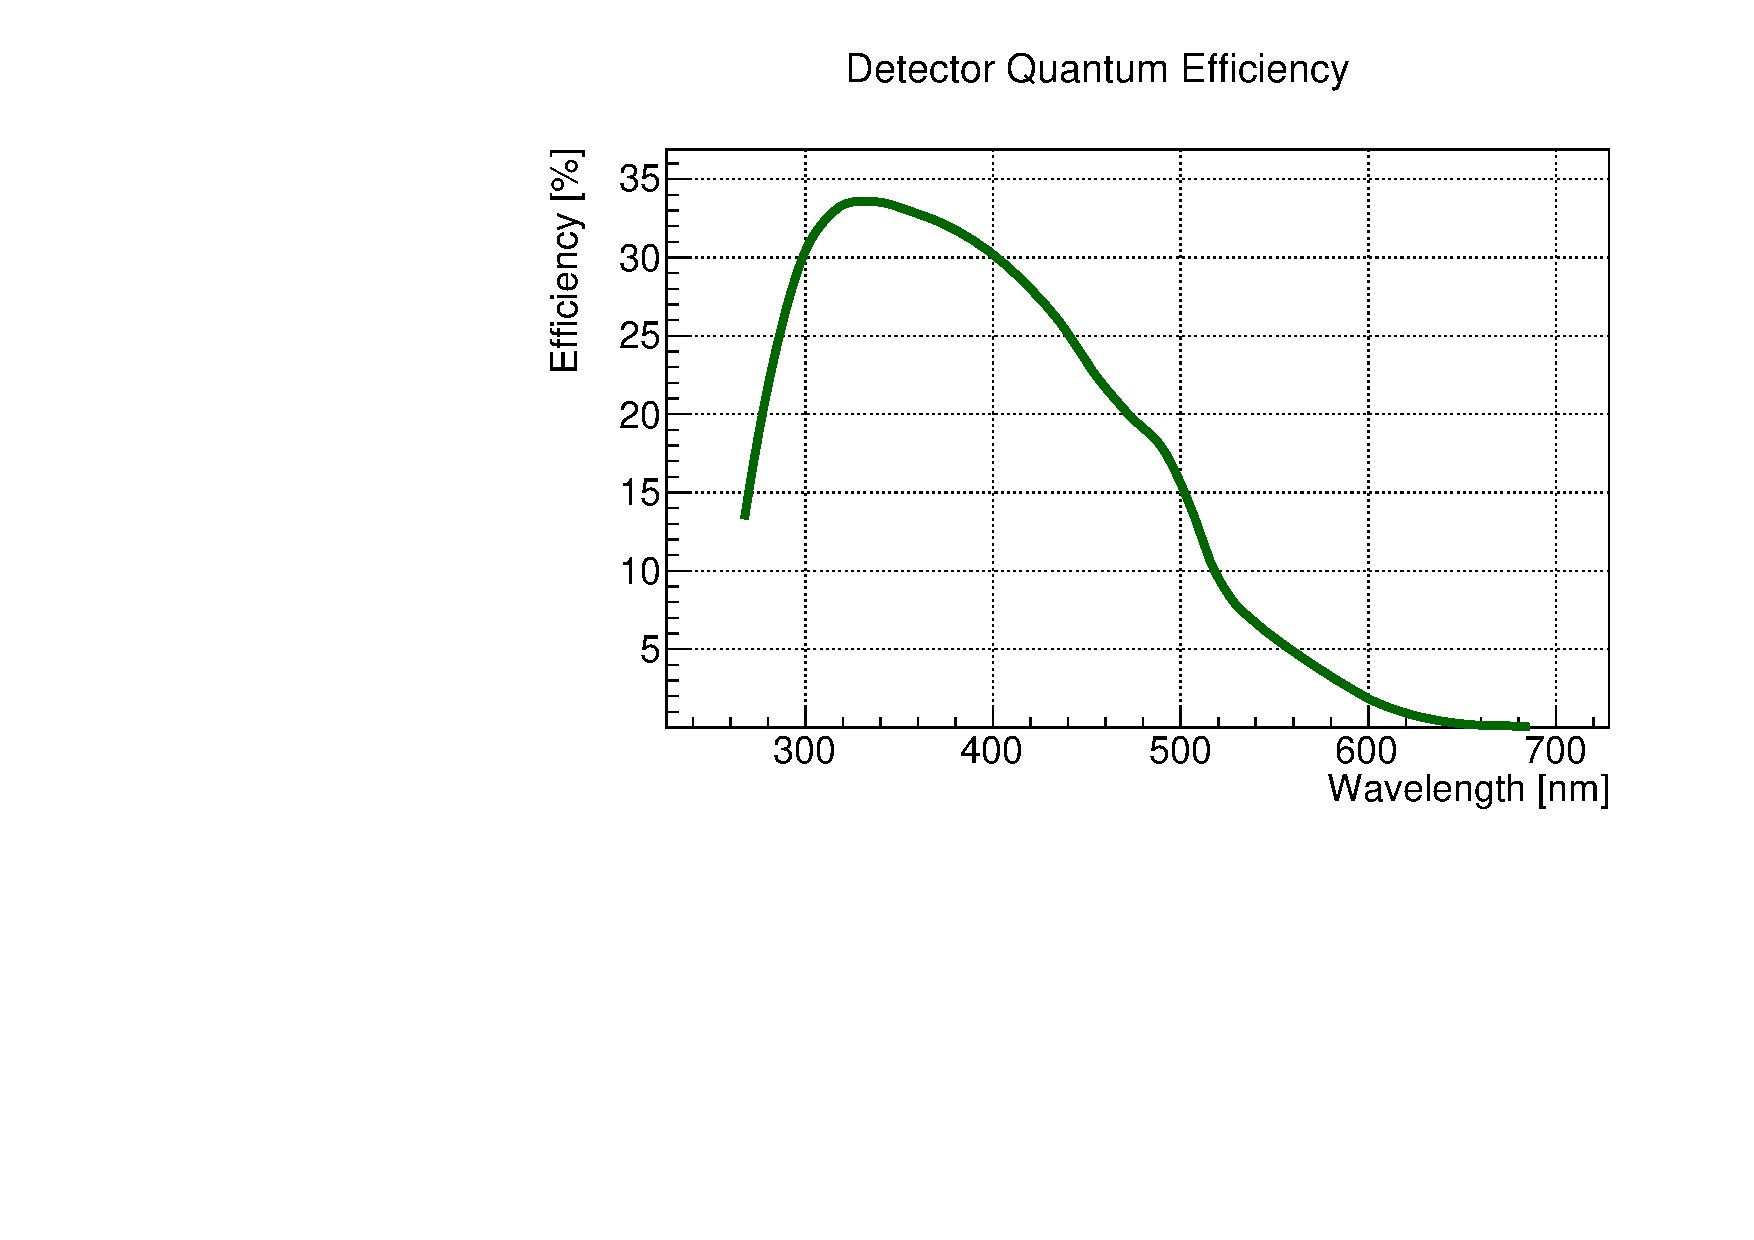
\includegraphics{./figs/qEff.pdf}}
\caption[Quantum Efficiency of H12700 PMT used by EMPHATIC.]{Quantum Efficiency of H12700 PMT used by EMPHATIC.}
\label{fig:qEff} 
\end{figure}

From equation \ref{eq:frankTamm}, we see that the distribution of photon wavelengths follows the distribution $1/\lambda^2$, so each photon is produced with a wavelength randomly drawn from this distribution on a range from 250 nm to 695 nm.
These values were chosen, because if we linearly extrapolate the quantum efficiency curve, we see that we do not expect to get any detector response for photons of wavelengths outside of this range.
Because all optical processes included in this simulation are inelastic, we do not expect any photon wavelength to change between the point of generation and the point of detection.
Therefore, after generating Cherenkov photons we may randomly reject them immediately based on their probability of being detected, and not simulate their paths any further.

The PMTs have dimensions of 48.5 mm $\times$ 48.5 mm.
Each PMT contains $8 \times 8$ pixels, and have a packing density of 87\%. 
The PMTs are expected to be arranged onto a 30 cm $\times$ 30 cm plane with a packing efficiency of $80\%$, 20 cm downstream of the first layer of aerogel.
\TODO{Find out where packing efficiency of 0.8 comes from}.
To model the photon detector array, we simply project the photons downstream onto a 30 cm $\times$ 30 cm histogram with $48 \times 48$ bins.
The number of photons counted in each bin is scaled by a factor of $80\% \times 87\%$ to account for the packing efficiencies.

Two examples of photon distribution arising from this simple simulation are shown in Figure \ref{fig:noScat}. While this simulation well approximates the expected location of a particle's photon rings for a single layer of aerogel, it is missing a number of key effects that would allow it to actually be used to calculate a realistic photon distribution.


\begin{figure}[]
  \centering
  \subfloat[Centered beam.]{\includegraphics[width=0.45\textwidth]{./figs/noscatter.pdf}\label{fig:f1}}
  \hfill
  \subfloat[Beam at an angle of 0.44 radians off the $z$-axis]{\includegraphics[width=0.45\textwidth]{./figs/noscatterangle.pdf}\label{fig:f2}}
  \caption{ Examples of two photon distributions \TODO{Redo these two figures: Make them the same dimension, and tall so that they can be placed side by side}}
  \label{fig:noScat}
\end{figure}

\section{Optical Effects}
Following this initial simulation, more sophisticated optical effects were added in. 

\subsection{Aerogel Choice}


$d1*tan(acos(1.0/n1)) = d2*tan(acos(1.0/n2)) $

\subsection{Rayleigh Scattering}

For EMPHATIC, aerogels with indices of refraction ranging from 1.03 to 1.05 in increments of 0.005 were considered, each with a thickness of 2 cm.
The properties of different typical aerogels were characterized by another member of the collaboration \TODO{give credit to Tabata}: their refractive indices were measured for light with a wavelength of 405 nm, and the transmittances of light were measured for light of wavelengths ranging from 190 nm to 800 nm.
The transmittance and refractive index of each aerogel are shown in Figure \TODO{aerogel refractive indices}.

As described in Section \ref{sec:optics}, the primary optical effect to account for is Rayleigh Scattering, wherein photons scatter with a probability proportional to $\lambda^{-4}$, and in a direction proportional to $1 + \cos^2(\theta)$.
If we assume that the transmittance of light through the aerogels is only affected by Rayleigh scattering then we can approximate $L(\lambda)$, the Rayleigh scattering interaction length at each wavelength, with the following formula:

\begin{equation}
L(\lambda) = \frac{-d}{\log(T(\lambda))}
    \label{eq:scatLength}
\end{equation}

In this equation, $T(\lambda)$ is the transmittance of light at a wavelength $\lambda$ across some thickness $d$ of the aerogel.
In order to efficiently sample a random distance before scattering, we can apply inverse transform sampling \TODO{Cite inverse transform sampling}.
The probability $p$ that a photon has scattered after travelling some distance $x$ through the aerogel is given by

\begin{equation}
p = 1 - \exp(-x/L)
    \label{eq:scatProb}
\end{equation}

To randomly draw a distance $x$ from this distribution, we can sample some $p$ uniformly on the range $[0,1]$, and get a distance $x$ by calculating the inverse:

\begin{equation}
x =   -L\ln(1-p)
  \label{eq:randomScat}
\end{equation}

In the simulation, when each photon is generated, a random ``distance until scattering" is calculated this way. 
We check whether or not a photon would still be in the aerogel after having travelled that distance: if it is, then we advance it forwards by that amount, and then assign the photon a new direction, where $\theta$ is sampled from the distribution $1 + \cos^2(\theta)$, and $\phi$ is randomly sampled from $[0, 2\pi]$.
After the position and direction of the photon has been updated, a new ``distance until scattering" is calculated and this process is repeated. 
If we determine that a photon would not be in the aerogel after having travelled that distance, then we advance the photon forwards until the boundary of the aerogel.
We then check what material the photon would be entering, and update the direction of the photon to account for the refraction caused by the photon travelling between two mediums of different refractive indices.

%  \TODO{Cite https://www.osapublishing.org/josaa/fulltext.cfm?uri=josaa-29-7-1356&id=238954}.
In order to compute refraction, we can use the following equation: \TODO{cite}
\begin{equation}
\bf{s'} = \mu\bf{s} + \bf{g}\sqrt{1 - \mu^2[1-(\bf{g \dot s})^2]} - \mu \bf{g}(\bf{g \dot s})
\label{eq:refract}
\end{equation}

In this equation, $\mu$ is the ratio $n_1/n_2$, $\bf{s}$ is the unit direction of the incident photon, $\bf{g}$ is the unit normal vector pointing out of the aerogel slab the photon is exiting, and $\bf{s'}$ is the unit vector direction of the photon after being refracted.

After adding in these optical effects, An example of a photon distribution is shown in Figure \ref{fig:photonHist}.

\begin{figure}[]
\centering
\resizebox{0.9\textwidth}{!}{\includegraphics{./figs/photonHist.pdf}}
\caption[Example of simulated photon distribution for centered 7.0 GeV pion beam]{Histograms displaying the simulated photon distribution for a 7.0 GeV pion beam travelling directly along the $z$-axis. Clockwise, from bottom left: (1) histogram of mean detected photon count per pixel on detector plane, (2) $y$-axis projection of photon distribution, (3) histogram of photon detections as function of distance from origin, (4) $x$-axis projection of photon distribution. }
\label{fig:photonHist} 
\end{figure}


\section{Comparison with Geant4} 
In this section, I will compare the simulated photon distribution between my simulation and the full Geant4 simulation.
They will be compared on a number of metrics, including the number of photons detected in the photon ring, and the level of background photons (determined by taking the ratio of histograms simulated by my simulation and by Geant4). This work is in progress: comparisons have been done, but it is still necessary to more accurately quantify the differences between the two simulations and display these results. I will describe the differences between my simulation and the full Geant4 simulation, and make the claim that my simulation contains enough of the necessary physics to simulate Cherenkov photons with sufficient accuracy for our purposes.

\section{Mirror?}

\endinput

Any text after an \endinput is ignored.
You could put scraps here or things in progress.

%% The following is a directive for TeXShop to indicate the main file
%%!TEX root = diss.tex

\chapter{Results}
\label{ch:Results}

\section{Fast Simulation Performance}
It was found that the fast ARICH simulation takes approximately 4 seconds to generate a photon distribution resulting from simulating 10,000 particles when running on a computer with a 2.7 GHz processor. 
Simulating the same 10,000 particles on the same computer using the Geant4 simulation of the EMPHATIC setup took approximately 100 seconds.
By ignoring all irrelevant physical processes in the simulation and removing the majority of the overhead of a Geant4 simulation, a significant performance speedup was attained.

\section{Particle Separation}
It is necessary to establish the effectiveness of the likelihood particle identification technique under different conditions.
As an example, let us suppose we want to determine how well this likelihood approach works on a particle that is 7 GeV and measured to enter the center of the aerogel and travel directly in the $z$-direction.
To check the certainty with which this technique can identify whether this is a pion or kaon, I applied the following procedure:

\begin{enumerate}
\item Generate 10,000 pions with the given position, direction, and momenta in Geant4, project the generated Cherenkov photons onto a plane representing the detector, apply efficiency corrections, and store the resulting histogram of detected photon hits for each pion. 
\item Do the same, but with simulated kaons instead of pions.
\item Given the particle initial position, initial direction, and momentum, use the fast ARICH simulation to generate two photon probability distribution histograms, corresponding to pions or kaons.
\item For each event simulated using Geant4, compute the negative log-likelihood of the event histogram with respect to the photon probability distribution functions of each particle hypothesis.
\item For each true particle type, plot a histogram of the log of the ratio of likelihoods between the two hypotheses.
This is just the differences between the negative log-likelihoods of the two hypotheses.
\item Look at the separation between the distributions: this is equal to the difference in means between the distributions, divided by the root mean square of each distribution added in quadrature
\end{enumerate}

The result of this procedure is shown in Figure \ref{fig:kaonpionsep}. The two distributions are separated by a distance of $1.9 \sigma$ - the significant overlap between the two distribution indicates that there is some chance of misidentification. Applying the same procedure to verify the separation between kaons and protons gives the results shown in Figure \ref{fig:kaonprotonsep}. Here we see that the two distributions do not significantly overlap and have a separation of $4.7 \sigma$, meaning that at this momentum and angle, protons are very unlikely to be misidentified as kaons, and vice versa.
\begin{figure}[]
\centering
\resizebox{0.9\textwidth}{!}{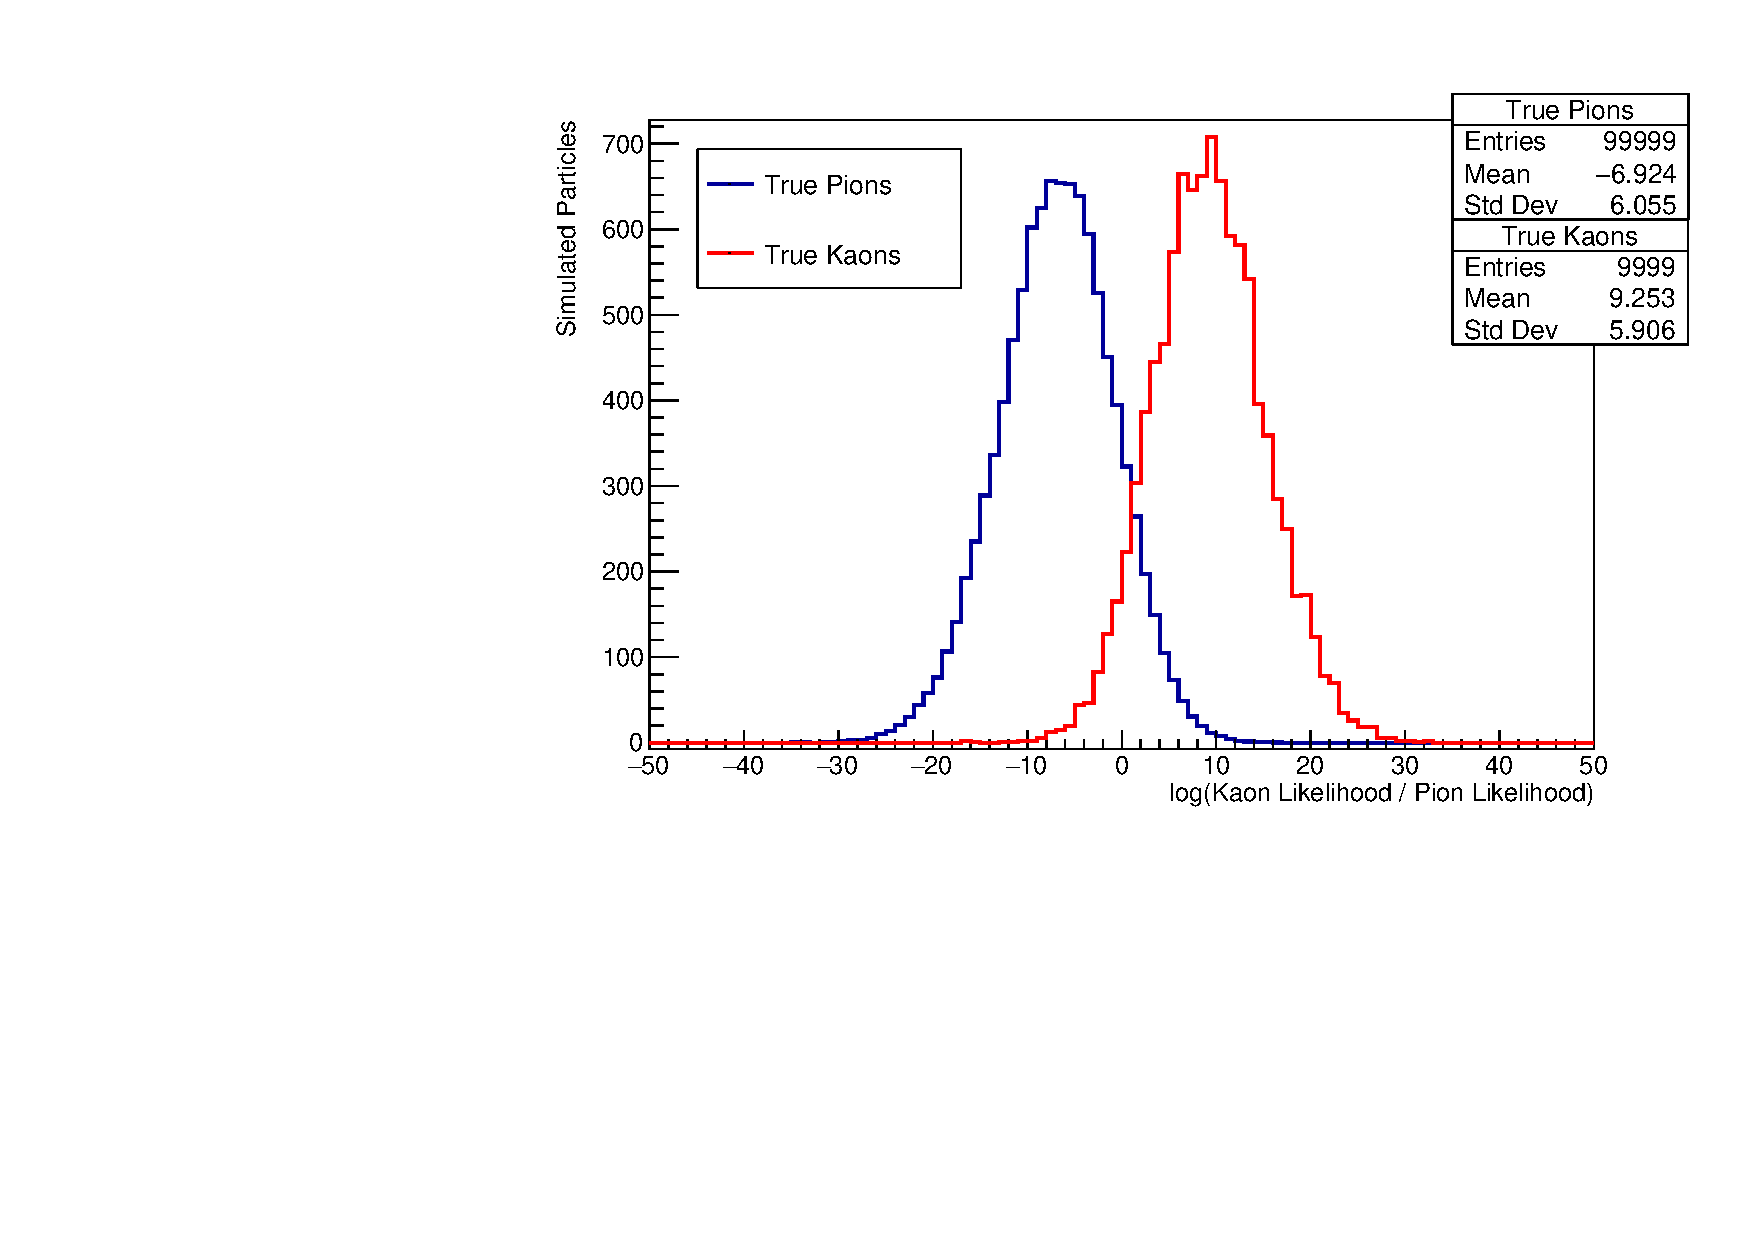
\includegraphics{./figs/kaonPionSep.pdf}}
\caption[Particle identification separation for 7 GeV/c pions and kaons]{Histogram showing the logarithm of the ratios of likelihoods between 7 GeV/c kaons and pions for both ``true" kaons and ``true" pions. The two distributions have a separation of 1.9 $\sigma$.}
\label{fig:kaonpionsep} 
\end{figure}

\begin{figure}[]
\centering
\resizebox{0.9\textwidth}{!}{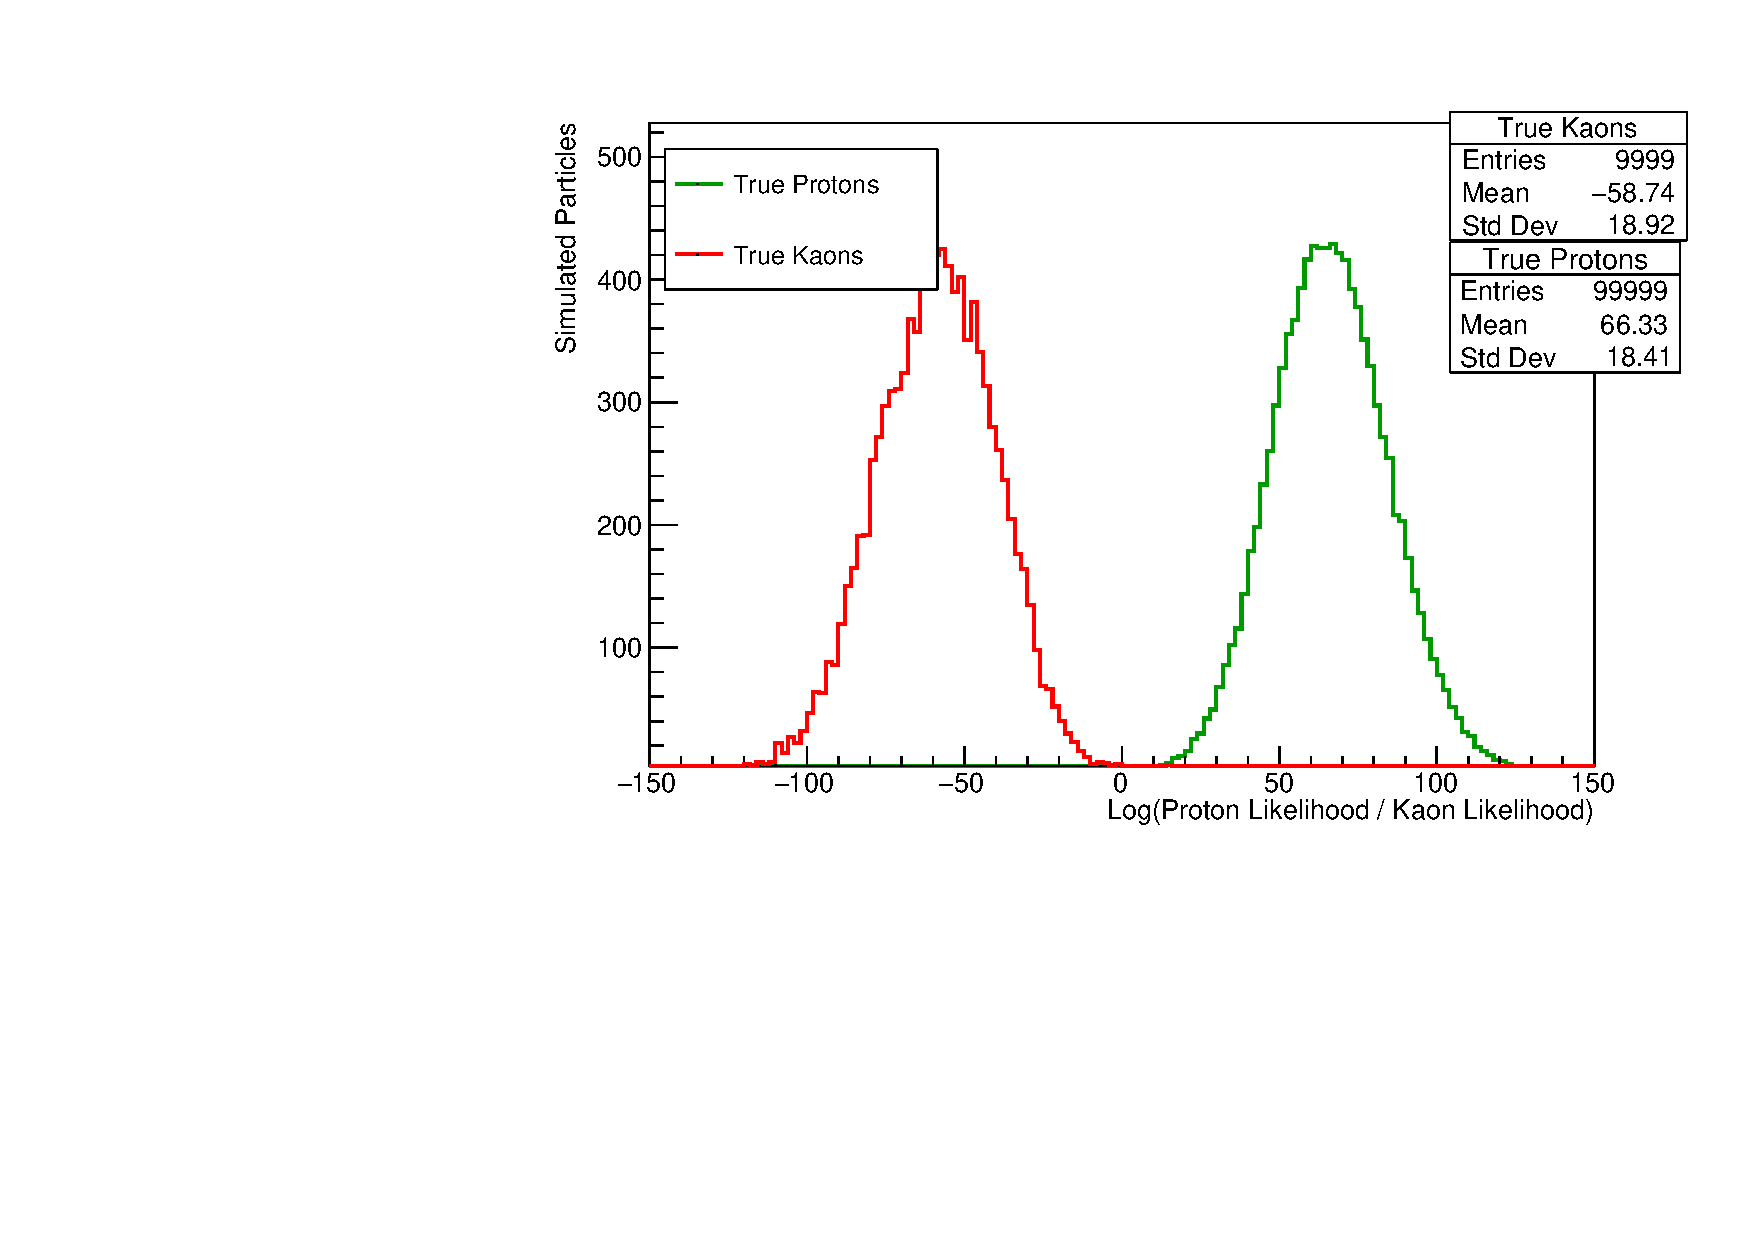
\includegraphics{./figs/kaonProtonSep.pdf}}
\caption[Particle identification separation for 7 GeV/c kaons and protons]{Histogram showing the logarithm of the ratios of likelihoods between 7 GeV/c protons and kaons for both ``true" protons and ``true" kaons. The two distributions have a separation of  4.7 $\sigma$.}
\label{fig:kaonprotonsep} 
\end{figure}

\subsection{Momenta}

At increasing momenta, it becomes increasingly hard to distinguish between particles, as their velocities converge to $c$ and their Cherenkov angles in a given aerogel converge to the same value. 
This can be seen in Figure \ref{fig:changles}, which plots the Cherenkov angles of different particles as a function of their momentum.
It is particularly hard to distinguish between pions and kaons, but easier to distinguish protons from kaons, and easier still to distinguish protons from pions.

\begin{figure}[]
\centering
\resizebox{0.9\textwidth}{!}{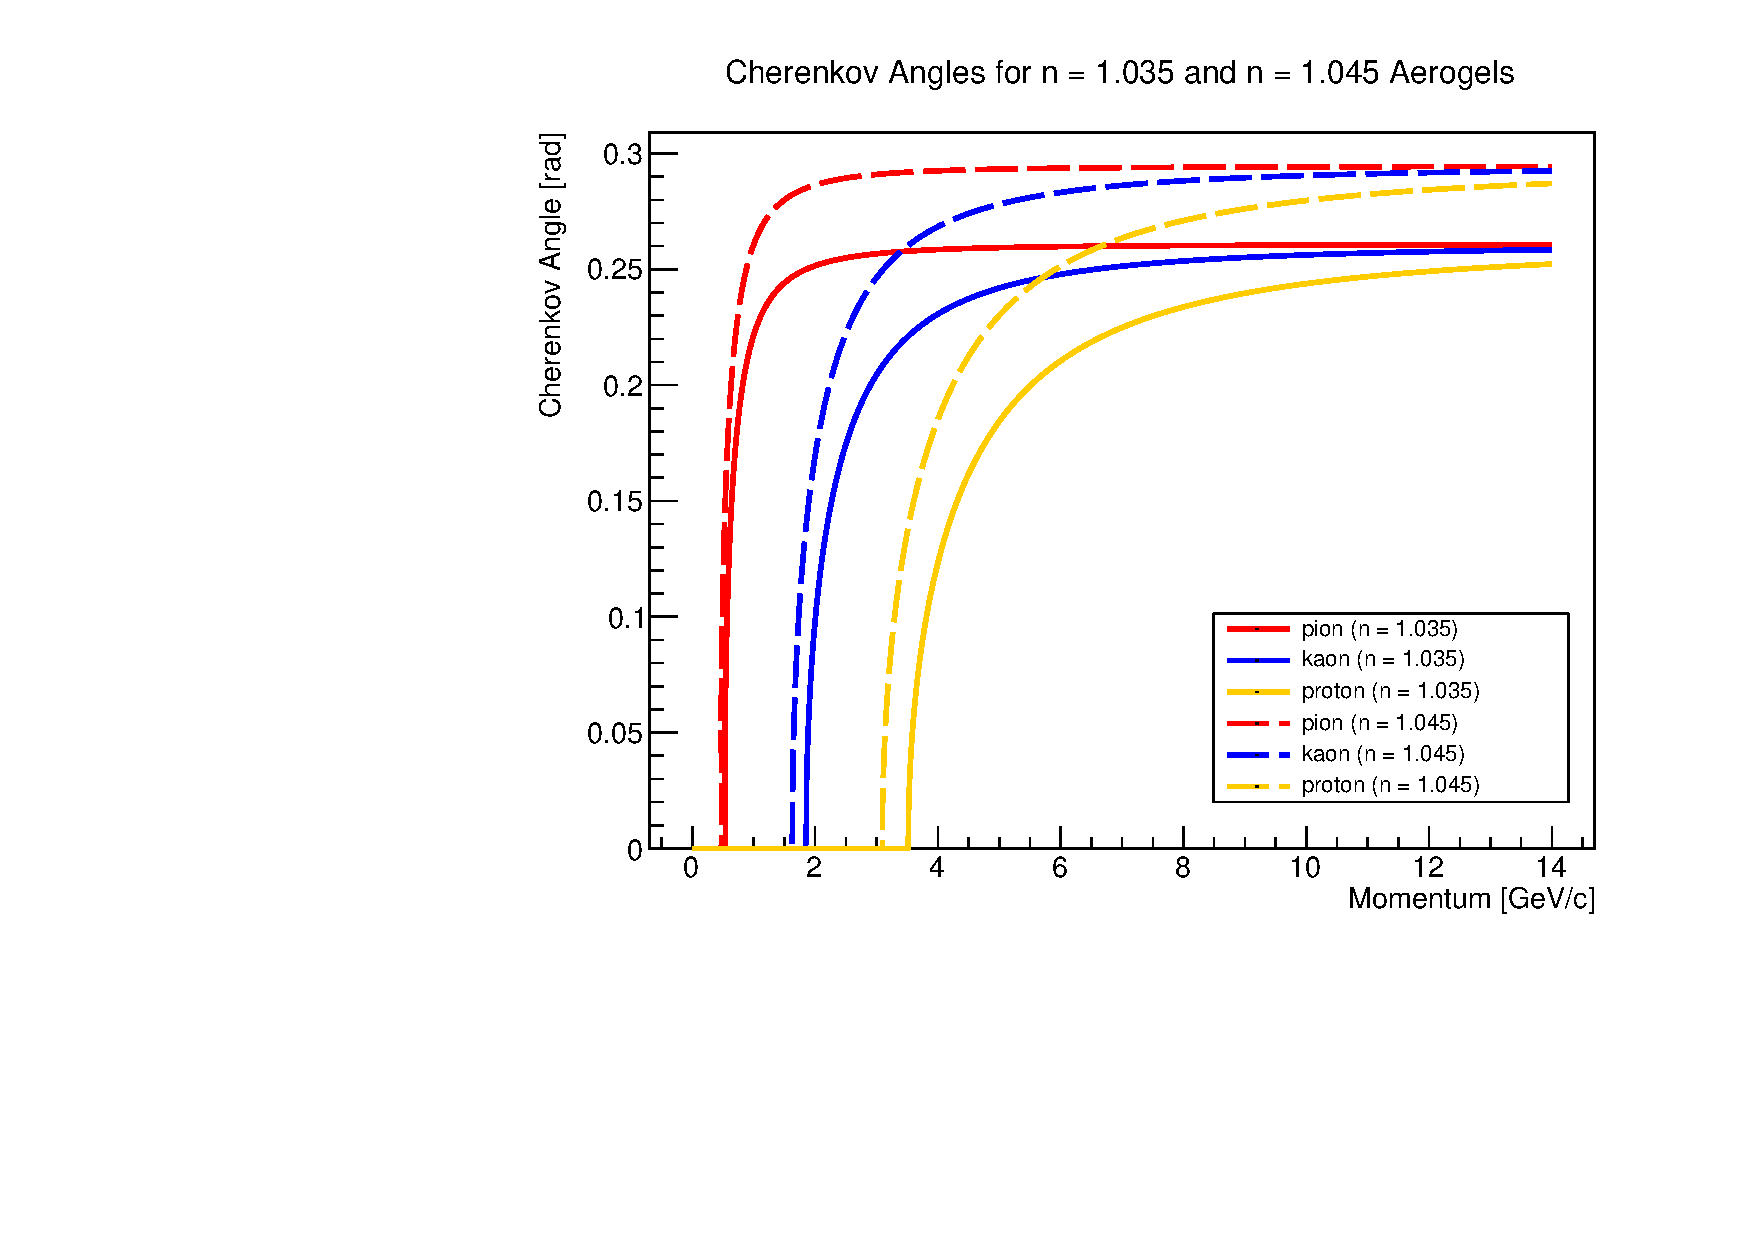
\includegraphics{./figs/changles.pdf}}
\caption[Predicted Cherenkov angles of pions, kaons, and protons over a range of momenta.]{Predicted Cherenkov angles of pions, kaons, and protons over a range of momenta.}
\label{fig:changles}
\end{figure}


A script was written to automate this procedure over a range of different initial particle directions and particle momenta. 
Figure \ref{fig:centeredSeps} shows the separation between likelihood distributions for each particle-particle pair over a range of momenta from 6 GeV/c to 14 GeV/c, with particles travelling directly down the $z$-axis.
The effectiveness of this technique for particle separation can also be measured by looking at misidentification rates: that is, the percentage of the time the particle identity that yielded the minimum negative log-likelihood among the candidate particles was not the true particle.
This is shown in Figure \ref{fig:centeredMis}.

\begin{figure}[]
\centering
\resizebox{0.9\textwidth}{!}{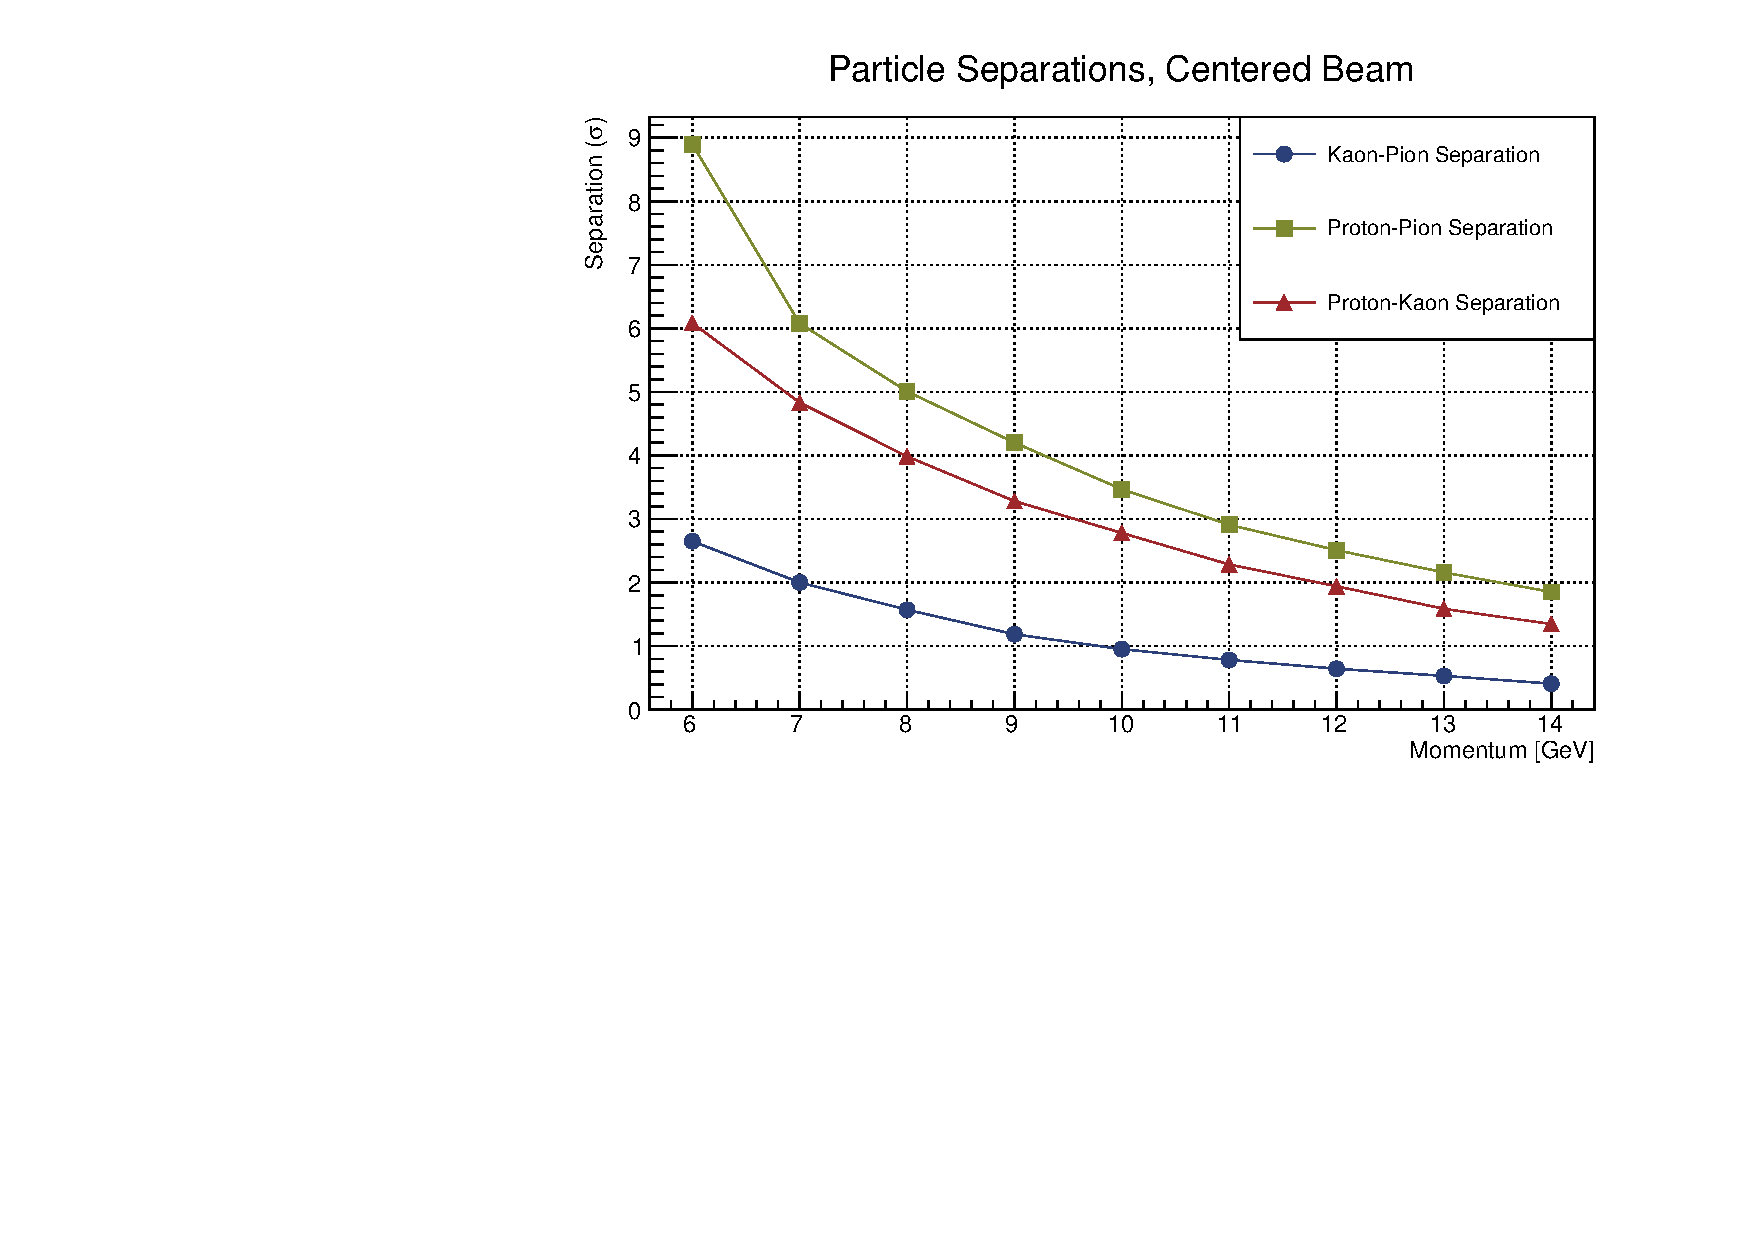
\includegraphics{./figs/centeredSeps.pdf}}
\caption[Plot of the separation between the distributions of computed log-likelihood ratios of different particle pairs, over a range of momenta. ]{Plot of the separation between the distributions of computed log-likelihood ratios of different particle pairs, over a range of momenta. Each ``true" particle was simulated 10,000 times using the Geant4 simulation as entering the aerogel layers with an angle $\theta = 0$ with respect to the downstream axis.}
\label{fig:centeredSeps} 
\end{figure}

\begin{figure}[]
\centering
\resizebox{0.9\textwidth}{!}{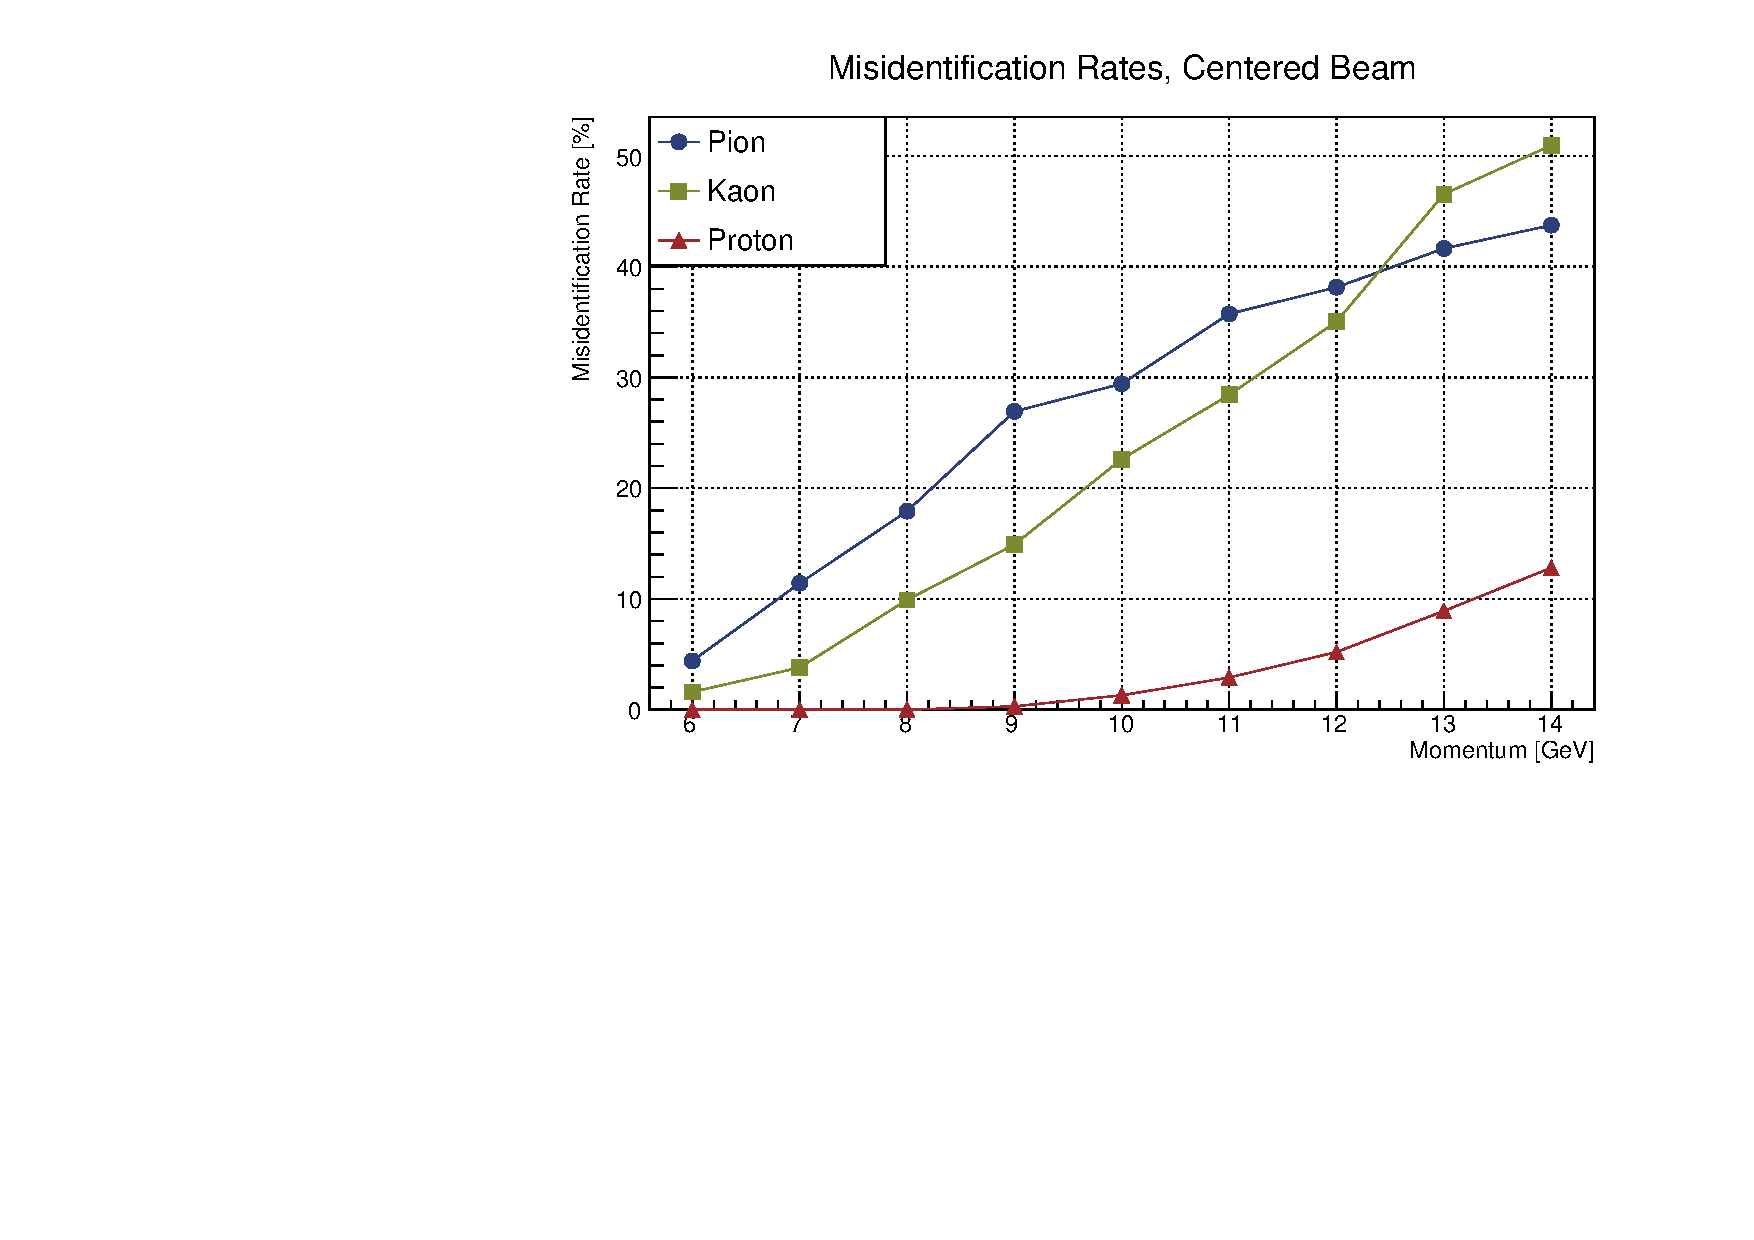
\includegraphics{./figs/centeredMisidentification.pdf}}
\caption[Plot of misidentification rate of the likelihood approach to particle identification over a spectrum of momenta.]{Plot of misidentification rate of the likelihood approach to particle identification over a spectrum of momenta. Each ``true" particle type was simulated 10,000 times using Geant4, and were simulated as entering the aerogel layers with an angle $\theta = 0$ with respect to the downstream axis.}
\label{fig:centeredMis} 
\end{figure}

We see that as momentum increases, we steadily become less effective at distinguishing between pions and kaons - we get a separation greater than $2 \sigma$ past momenta of 7 GeV/c, and at a momentum of 14 GeV/c, we do no better than chance at determining whether a particle is a kaon or pion.
We see that protons remain easily distinguishable from pions and kaons we reach approximately 12 or 13 GeV/c respectively. 

\subsection{Angles}
When particles enter the aerogel at nonzero angles with respect to the beamline axis, a number of intractable effects affect the resulting photon distribution. 
Particles travel further through the aerogel at higher angles and may produce more photons, photons refract differently at higher angles, and the resulting Cherenkov cones may become smeared out over more PMT pixels. 
To evaluate the effectiveness of this likelihood approach across different angles, the procedure described in the preceding section was followed over 5 angular bins ranging from 0 to 0.4 radians.
The resulting particle separations are shown in Figure \ref{fig:angleSeps}.

It is clear that as the angle of the incident particle increases, we become better able to separate out our particles from one another up until a certain point.
This is likely because the photon rings are ``smeared out" over several different PMT pixels, allowing for finer details to be measured. 
However, past 0.35 radians we see that our ability to distinguish particles significantly decreases.
This is because at this point, the photon rings partially fall off of the detector plane, and with fewer detected photons, there is less information to distinguish particles.

\begin{figure}[]
\centering
\resizebox{0.9\textwidth}{!}{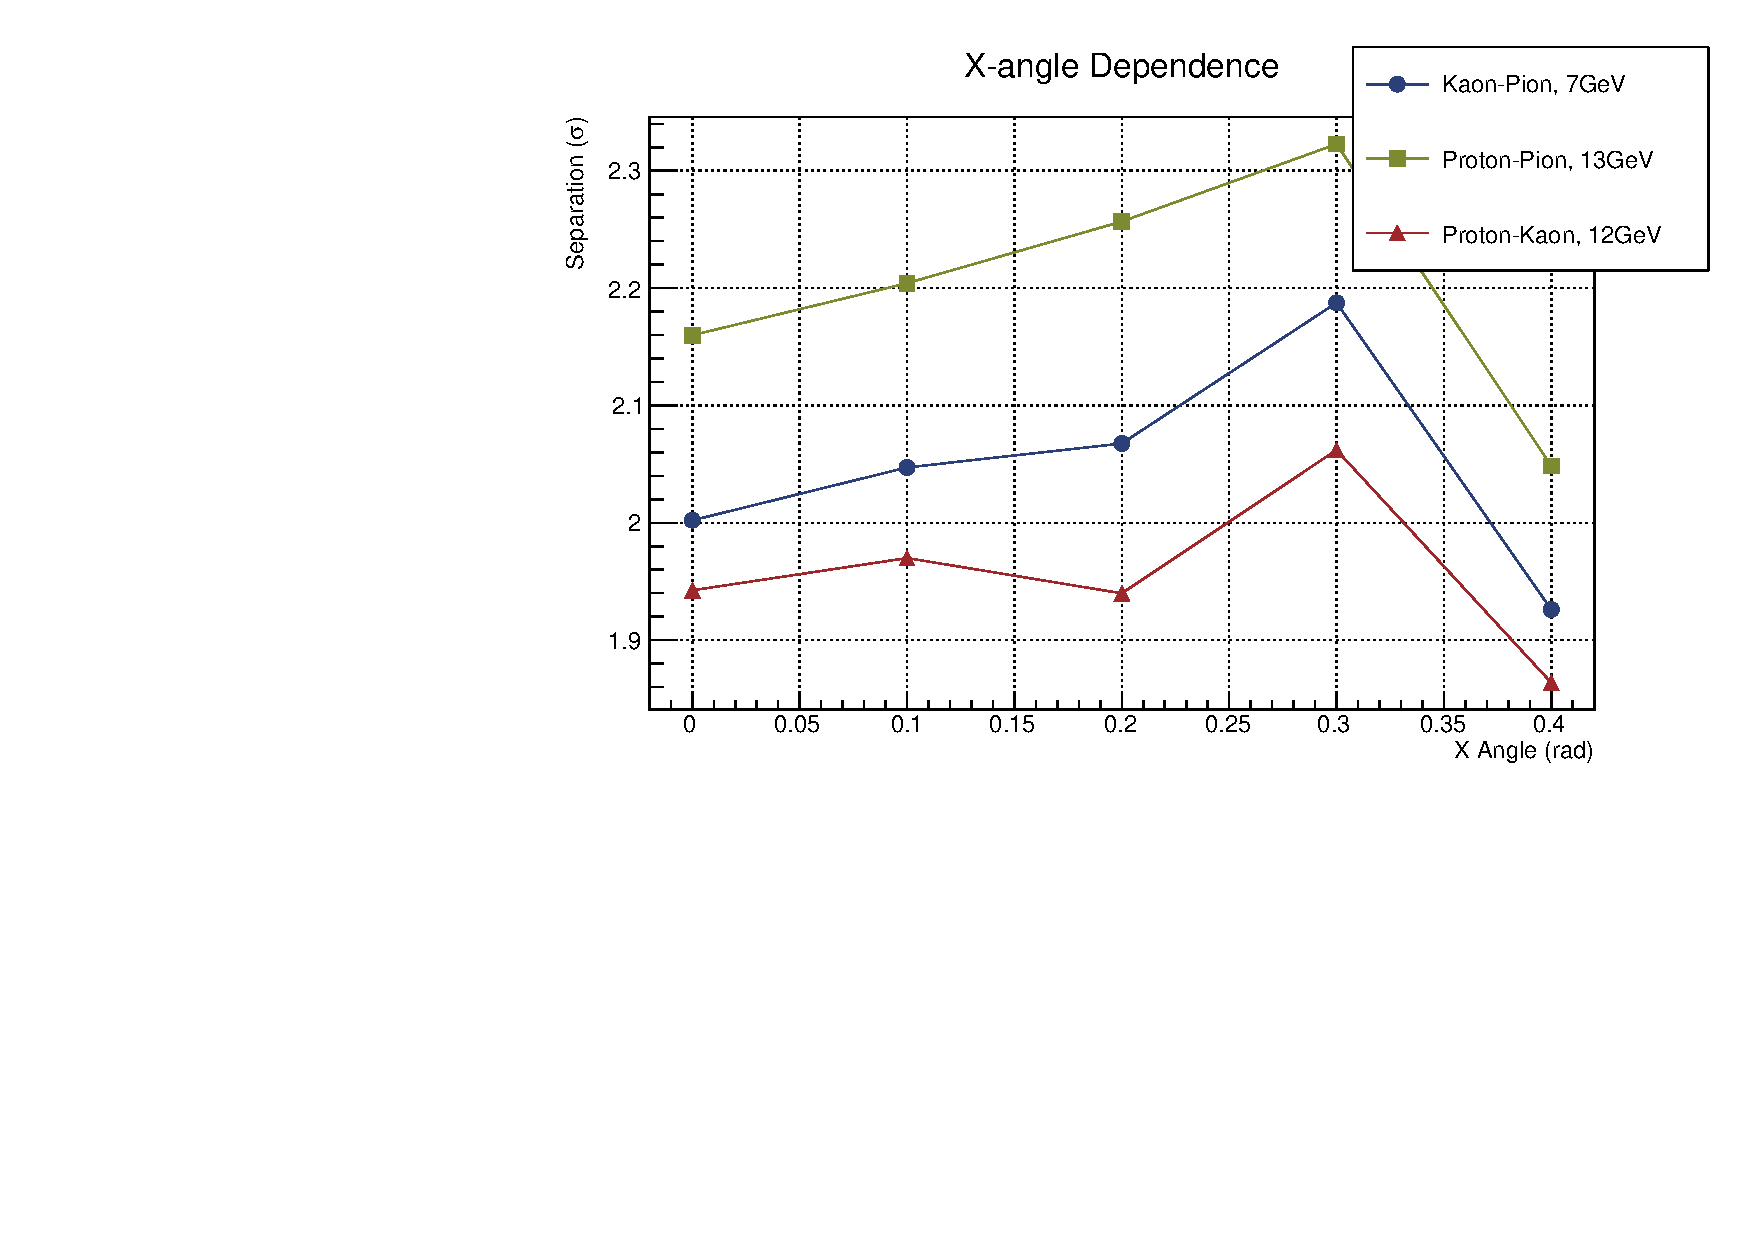
\includegraphics{./figs/xAngleSeps.pdf}}
\caption[Plot of the separation between the distributions of computed log-likelihood ratios of different particle pairs, over a range of angles. ]{Plot of the separation between the distributions of computed log-likelihood ratios of different particle pairs, over a range of angles. Each particle is simulated 10,000 times using the Geant4 simulation as entering the aerogel layers with an angle with respect to the downstream axis. \TODO{reword this}}\label{fig:angleSeps}
\end{figure}


\section{Multi-particle events}
\label{sec:multiparticle}
Although so far only single-photon ring events have been evaluated, it is often the case that the photons from several different particles will be detected at the same time in the ARICH detector. 
It is necessary that the likelihood particle identification technique is able to separate out multi-particle events as well. 

To accomplish this, the simulation was modified to take in an array of different particle momenta, positions, and directions, rather than just one set of parameters.
Because the photon rings from each particle may overlap with one another and cannot necessarily be disentangled, every possible combination of particle hypotheses must be simulated and compared to the event data in order to concurrently fit all particles.
Because the photon probability distribution functions for each particle are independent, each particle is independently simulated for each particle hypothesis, and the resulting photon histograms are saved.
Next, for every possible combination of these particle hypotheses, we sum together the corresponding particles' photon distribution histograms and calculate a log-likelihood by comparing the sum to the event data.
In total, for $n$ detected particles and $p$ possible particle hypotheses, we must simulate $p \times n$ photon distribution functions, do $p^n$  log-likelihood comparisons with our event data, and select the combination with the minimum negative log-likelihood from these $p^n$ options. 

An example of the result of this process demonstrated in Figure \ref{fig:multiParticle}. A three-particle event was simulated, consisting of one kaon, one pion, and one proton. 
Each particle had a momentum randomly drawn from a Gaussian with a mean of $10$ GeV/c and a standard deviation of $2$ GeV/c, with directions thrown from a Gaussian with a mean of $0$ rad and standard deviation of $0.3$ rad, and with initial positions drawn from a Gaussian with a mean of $0$ and a standard deviation of $2$ cm.
The values for their momenta, positions, and directions were then used as inputs to the fast simulation, and the likelihoods of each of the 27 possible particle combinations were calculated.
In this particular example, the particle identification code was able correctly the identify the ``true" combination of particle types.
However, this was an arbitrary test - real experimental data would not necessarily resemble distributions such as this.

\begin{figure}[]
\centering
\resizebox{0.9\textwidth}{!}{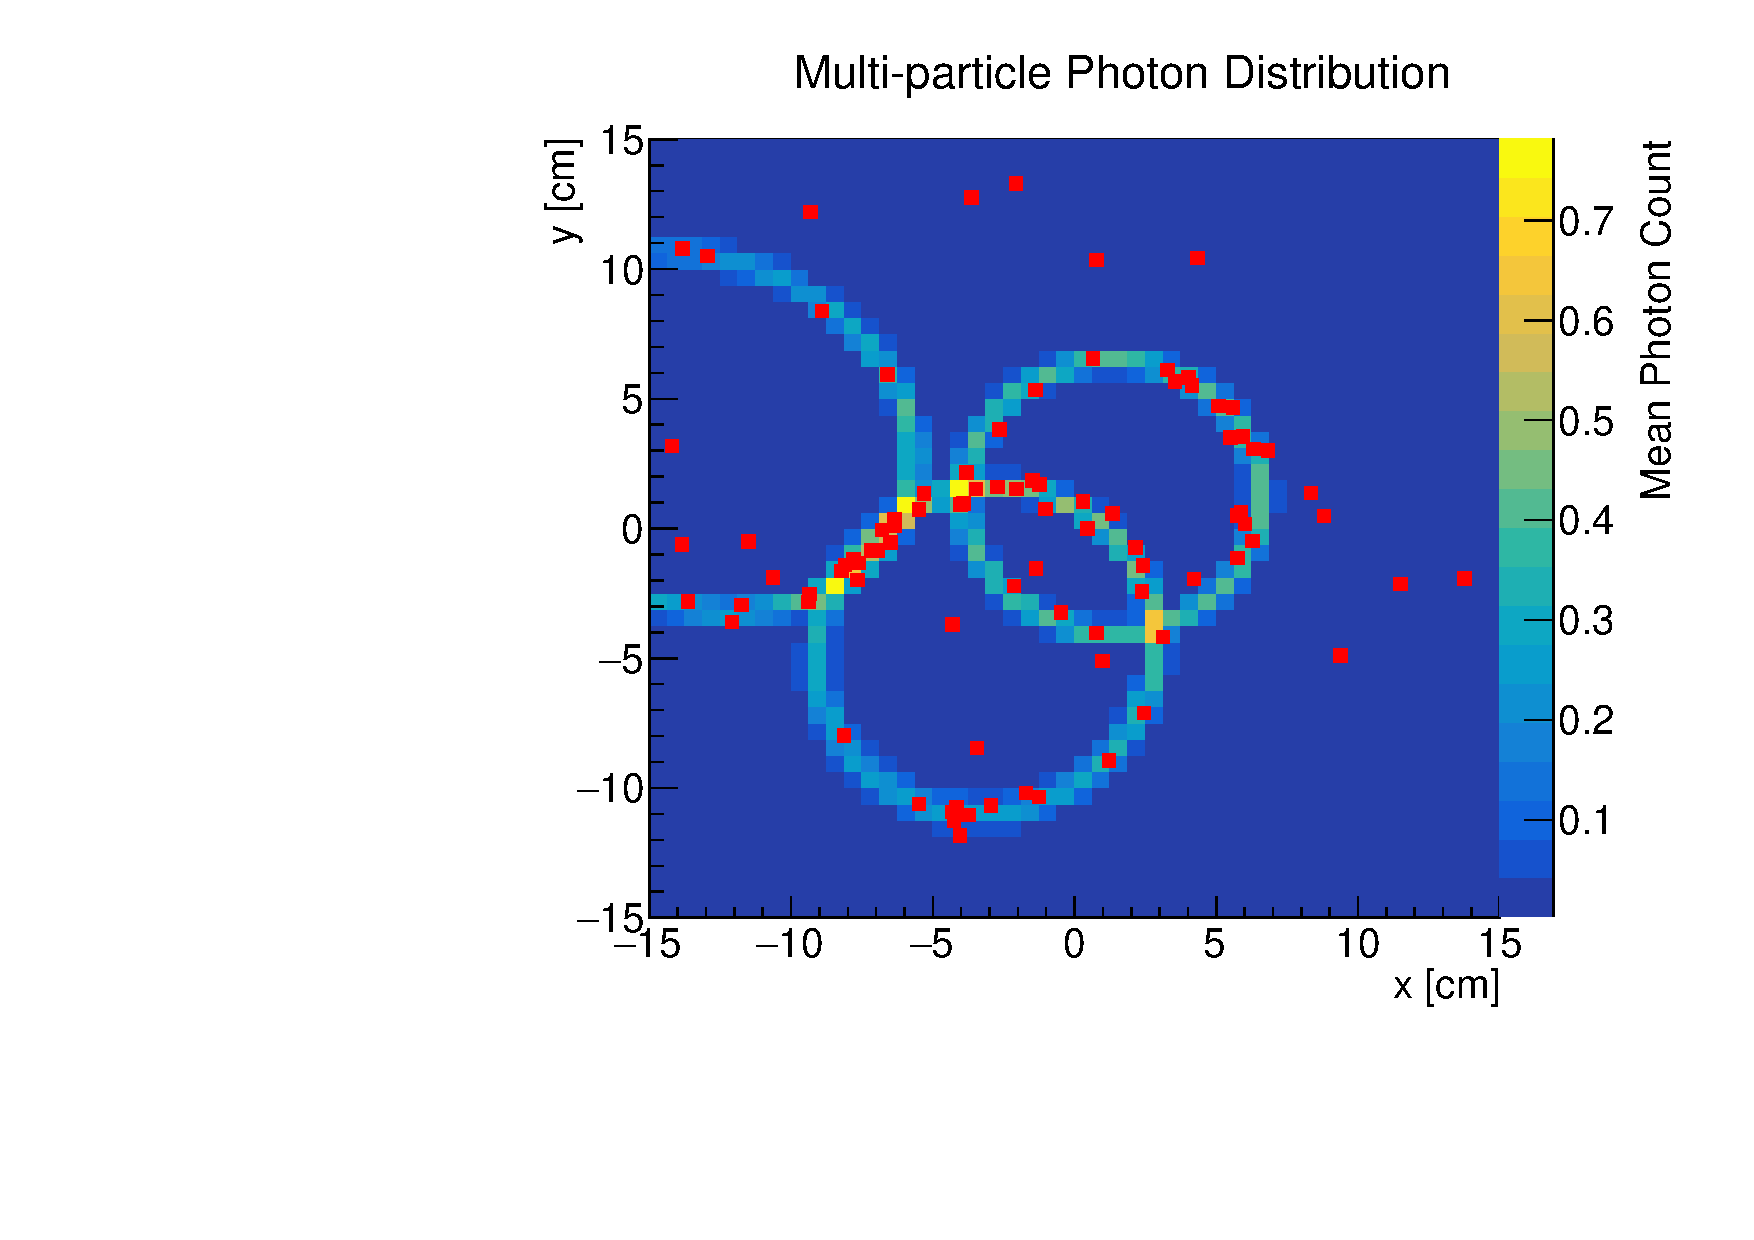
\includegraphics{./figs/pdfMultiParticle.pdf}}
\caption[Simulated event data and expected photon distribution for a three-particle event]{Histogram of photons detected in a simulated event (shown in red) overlaid on the photon distribution of the best-fit particle hypothesis for the data, corresponding to a pion, a kaon, and a proton.}
\label{fig:multiParticle} 
\end{figure}


\endinput

Any text after an \endinput is ignored.
You could put scraps here or things in progress.

%% The following is a directive for TeXShop to indicate the main file
%%!TEX root = diss.tex

\chapter{Discussion}
\label{ch:Discussion}

The technique of using a likelihood method of  particle identification was found to be useful at distinguishing between lower momentum single-particle events.
However, several more cases and extensions must be examined to properly evaluate the usefulness of this technique for analyzing experimental data. 
These are discussed in this section. 

\section{Multi-Particle Events}
Although multi-particle fitting was implemented and briefly verified in Section \ref{sec:multi}, in order to get a useful measure of our ability to measure multi-particle events, it is necessary that we better understand what these events might look like in a real experiment.
We do not know the rate at which we see multi-particle events, and we do not know what particle species we would expect to see in coincidence with each other.
For instance, if we are likely to frequently see both high-momentum kaons as well as high-momentum pions, then we may encounter difficulty in fitting these photon rings.

To find out what these multi-particle events may look like in a typical experiment, we could use the Geant4 simulation of EMPHATIC to simulate a typical experiment.
Geant4 contains libraries to simulate elastic scattering, particle decays, hadron physics, stopping physics, Cherenkov radiation, and more, so such a simulation should well-approximate the types of events we would expect to see.
For instance, we could set up a simulation of protons colliding with a carbon target, apply our particle identification technique to the photon distributions of each event where multiple secondary charged particle enters the aerogel at a velocity sufficient to produce Cherenkov photons, and examine what events cause us to misidentify particles.
This would help inform us on the practical effectiveness of the method outlined in this report.

\section{High-Angle Photons}
As seen in Figure \ref{fig:angleSeps}, we lose the ability to distinguish between different particles when they enter the aerogel at sufficiently high angles, as the photon rings begin to fall out of the angular acceptance of the photon detector.
One proposed solution to this issue is the addition mirrors to the sides of the detector, which would reflect high-angle photons onto the PMT array. 
While this would allow us to identify high-angle particles, it would increase the background from Rayleigh-scatter photons, as we typically see a broad angular range of scattered photons.

This addition was incorporated as an optional parameter to the fast ARICH simulation has an added option to include these mirrors.
Photons that would ordinarily exit out of the sides of a defined 30 cm $\times$ 30 cm region get reflected back in.
While this has been fully implemented, it remains to be seen how this affects our ability to separate particles.
Determining effectiveness of this approach also depends on knowledge of what we expect to see in an experimental event - if high-angle particles are rare, the increases photon background may render this approach counterproductive.

\section{Momentum Error}
The particle identification method outlined so far involves fitting at the candidate particle velocities corresponding to the measured momentum of the unidentified particle.
However, this does not account for the resolution of the momentum measurements.
We may achieve a better fit for the simulated photon ring if the velocity of the simulated particle more closely matches the ``true" momentum of the particle, and get a more clear negative log-likelihood minima. 
To account for the resolution of the momentum measurements, we may simulate velocities corresponding not only to the measured momentum, but also at values equal to the measured momentum plus or minus one or two standard deviations.
We could then quadratically fit to obtain the specific expected velocity of the particle

This approach would likely be helpful for situations where the true velocity falls somewhere between the expected velocities for two different particle hypotheses for a measured momentum.  
However, this would yield three or five simulations per particle, rather than just one, significantly increasing the computation cost, especially for multi-particle events. 

\section{Further Extensions}
Several optical processes were ignored in the fast ARICH simulation, and adding these in may improve the particle fitting. 
Refraction was implemented at the boundaries between the two aerogels as well as the boundaries between aerogel and air, as these were thought to be the main processes altering the photon distributions.
Additional effects come from the reflection at the boundaries between media - this effect was assumed to have minimal impact, as the amplitude of the reflected light increases with respect to the angle of incidence with the boundary, and non-scattered photons that would make up the Cherenekov photon ring would have a relatively low angle.

In the fast simulation, the index of refraction of the aerogel was assumed to be constant for every wavelength of light.
However, this is a simplification: the refractive index decreases with increasing wavelength, and this effect must be experimentally measured to be parametrized \cite{aerogelrefrac}.

The current modelling of the detector is quite crude - a more sophisticated setup could be defined to account for the real dead space of the PMTs, the non-uniformity of their pixel size, and the glass boundary between the air and the PMT.

While all of the these modifications would increase the accuracy of the fast simulation, they would necessarily increase its runtime. 
Thus, each of these effects would have to be carefully assessed to determine whether the benefit in particle identification is sufficient to justify the increased computation time.

Each particle in the simulation is independent, so the simulation could potentially be modified to process each particle in parallel. 
Alternatively, because each experimental event is independent, this technique for particle identification could instead be sped up by processing each event in parallel.

\section{Alternate Approaches}
If it is determined that this Monte Carlo simulation-based likelihood approach to particle identification is too computationally expensive to perform, other approaches may be applied.
\TODO{Cite alternate approaches used by the BELLE II and LHC-B experiments}


\endinput 

Any text after an \endinput is ignored.
You could put scraps here or things in progress.



MULTIPARTICLE:

To find out what these multi-particle events may look like in a typical experiment, the Geant4 simulation of EMPHATIC was used to simulate a beam of 10,000 protons with a momentum of 30 GeV/c.
The protons were generated directly upstream of a 5.0 cm $\times$ 5.0 cm, 2.0 cm thick carbon target, and were directed along the $z$-axis of the experiment.
Geant4 libraries were included to account for elastic scattering, particle decays, hadron physics, stopping physics, and Cherenkov radiation, among other processes. 
The output of the simulation contains information about the identities and trajectories of the particles involved. 
Of interest to this project are specifically the instances where a secondary charged particle enters the aerogel at a velocity sufficient to produce Cherenkov photons.

\TODO{Include matrices of what particles we find as the highest-momentum particles vs. second-highest momentum particle. Key points: The most typical particle-particle combinations are higher-momenta protons with lower-momenta pions, or two pions.} 

It was found that out of the 10,000 events simulated, 24 contained positively charged Kaons entering the aerogel.
\TODO{If I have some time I'll look into the Kaon events.}


\include{conclusions}
% Generally recommended to put each chapter into a separate file
%\include{relatedwork}
%\include{model}
%\include{impl}
%%% The following is a directive for TeXShop to indicate the main file
%%!TEX root = diss.tex

\chapter{Discussion}
\label{ch:Discussion}

The technique of using a likelihood method of  particle identification was found to be useful at distinguishing between lower momentum single-particle events.
However, several more cases and extensions must be examined to properly evaluate the usefulness of this technique for analyzing experimental data. 
These are discussed in this section. 

\section{Multi-Particle Events}
Although multi-particle fitting was implemented and briefly verified in Section \ref{sec:multi}, in order to get a useful measure of our ability to measure multi-particle events, it is necessary that we better understand what these events might look like in a real experiment.
We do not know the rate at which we see multi-particle events, and we do not know what particle species we would expect to see in coincidence with each other.
For instance, if we are likely to frequently see both high-momentum kaons as well as high-momentum pions, then we may encounter difficulty in fitting these photon rings.

To find out what these multi-particle events may look like in a typical experiment, we could use the Geant4 simulation of EMPHATIC to simulate a typical experiment.
Geant4 contains libraries to simulate elastic scattering, particle decays, hadron physics, stopping physics, Cherenkov radiation, and more, so such a simulation should well-approximate the types of events we would expect to see.
For instance, we could set up a simulation of protons colliding with a carbon target, apply our particle identification technique to the photon distributions of each event where multiple secondary charged particle enters the aerogel at a velocity sufficient to produce Cherenkov photons, and examine what events cause us to misidentify particles.
This would help inform us on the practical effectiveness of the method outlined in this report.

\section{High-Angle Photons}
As seen in Figure \ref{fig:angleSeps}, we lose the ability to distinguish between different particles when they enter the aerogel at sufficiently high angles, as the photon rings begin to fall out of the angular acceptance of the photon detector.
One proposed solution to this issue is the addition mirrors to the sides of the detector, which would reflect high-angle photons onto the PMT array. 
While this would allow us to identify high-angle particles, it would increase the background from Rayleigh-scatter photons, as we typically see a broad angular range of scattered photons.

This addition was incorporated as an optional parameter to the fast ARICH simulation has an added option to include these mirrors.
Photons that would ordinarily exit out of the sides of a defined 30 cm $\times$ 30 cm region get reflected back in.
While this has been fully implemented, it remains to be seen how this affects our ability to separate particles.
Determining effectiveness of this approach also depends on knowledge of what we expect to see in an experimental event - if high-angle particles are rare, the increases photon background may render this approach counterproductive.

\section{Momentum Error}
The particle identification method outlined so far involves fitting at the candidate particle velocities corresponding to the measured momentum of the unidentified particle.
However, this does not account for the resolution of the momentum measurements.
We may achieve a better fit for the simulated photon ring if the velocity of the simulated particle more closely matches the ``true" momentum of the particle, and get a more clear negative log-likelihood minima. 
To account for the resolution of the momentum measurements, we may simulate velocities corresponding not only to the measured momentum, but also at values equal to the measured momentum plus or minus one or two standard deviations.
We could then quadratically fit to obtain the specific expected velocity of the particle

This approach would likely be helpful for situations where the true velocity falls somewhere between the expected velocities for two different particle hypotheses for a measured momentum.  
However, this would yield three or five simulations per particle, rather than just one, significantly increasing the computation cost, especially for multi-particle events. 

\section{Further Extensions}
Several optical processes were ignored in the fast ARICH simulation, and adding these in may improve the particle fitting. 
Refraction was implemented at the boundaries between the two aerogels as well as the boundaries between aerogel and air, as these were thought to be the main processes altering the photon distributions.
Additional effects come from the reflection at the boundaries between media - this effect was assumed to have minimal impact, as the amplitude of the reflected light increases with respect to the angle of incidence with the boundary, and non-scattered photons that would make up the Cherenekov photon ring would have a relatively low angle.

In the fast simulation, the index of refraction of the aerogel was assumed to be constant for every wavelength of light.
However, this is a simplification: the refractive index decreases with increasing wavelength, and this effect must be experimentally measured to be parametrized \cite{aerogelrefrac}.

The current modelling of the detector is quite crude - a more sophisticated setup could be defined to account for the real dead space of the PMTs, the non-uniformity of their pixel size, and the glass boundary between the air and the PMT.

While all of the these modifications would increase the accuracy of the fast simulation, they would necessarily increase its runtime. 
Thus, each of these effects would have to be carefully assessed to determine whether the benefit in particle identification is sufficient to justify the increased computation time.

Each particle in the simulation is independent, so the simulation could potentially be modified to process each particle in parallel. 
Alternatively, because each experimental event is independent, this technique for particle identification could instead be sped up by processing each event in parallel.

\section{Alternate Approaches}
If it is determined that this Monte Carlo simulation-based likelihood approach to particle identification is too computationally expensive to perform, other approaches may be applied.
\TODO{Cite alternate approaches used by the BELLE II and LHC-B experiments}


\endinput 

Any text after an \endinput is ignored.
You could put scraps here or things in progress.



MULTIPARTICLE:

To find out what these multi-particle events may look like in a typical experiment, the Geant4 simulation of EMPHATIC was used to simulate a beam of 10,000 protons with a momentum of 30 GeV/c.
The protons were generated directly upstream of a 5.0 cm $\times$ 5.0 cm, 2.0 cm thick carbon target, and were directed along the $z$-axis of the experiment.
Geant4 libraries were included to account for elastic scattering, particle decays, hadron physics, stopping physics, and Cherenkov radiation, among other processes. 
The output of the simulation contains information about the identities and trajectories of the particles involved. 
Of interest to this project are specifically the instances where a secondary charged particle enters the aerogel at a velocity sufficient to produce Cherenkov photons.

\TODO{Include matrices of what particles we find as the highest-momentum particles vs. second-highest momentum particle. Key points: The most typical particle-particle combinations are higher-momenta protons with lower-momenta pions, or two pions.} 

It was found that out of the 10,000 events simulated, 24 contained positively charged Kaons entering the aerogel.
\TODO{If I have some time I'll look into the Kaon events.}


%\include{conclusions}

%    3. Notes
%    4. Footnotes

%    5. Bibliography
\begin{singlespace}
\raggedright
%\bibliographystyle{abbrvnat}
\bibliographystyle{apsrev}
\bibliography{biblio}
\end{singlespace}

\appendix
%    6. Appendices (including copies of all required UBC Research
%       Ethics Board's Certificates of Approval)
%\include{reb-coa}	% pdfpages is useful here

\chapter{Simulation Code}

\TODO{
In this section, I will document the code: How to get it running, what inputs it takes in, what classes are included, and how each component interacts with one another. 
}

The full code repository is available at \url{https://github.com/danielTLevy/ARICHSim} \TODO{where do I link this from?}


\begin{sidewaysfigure}[]
\centering
\resizebox{1\textwidth}{!}{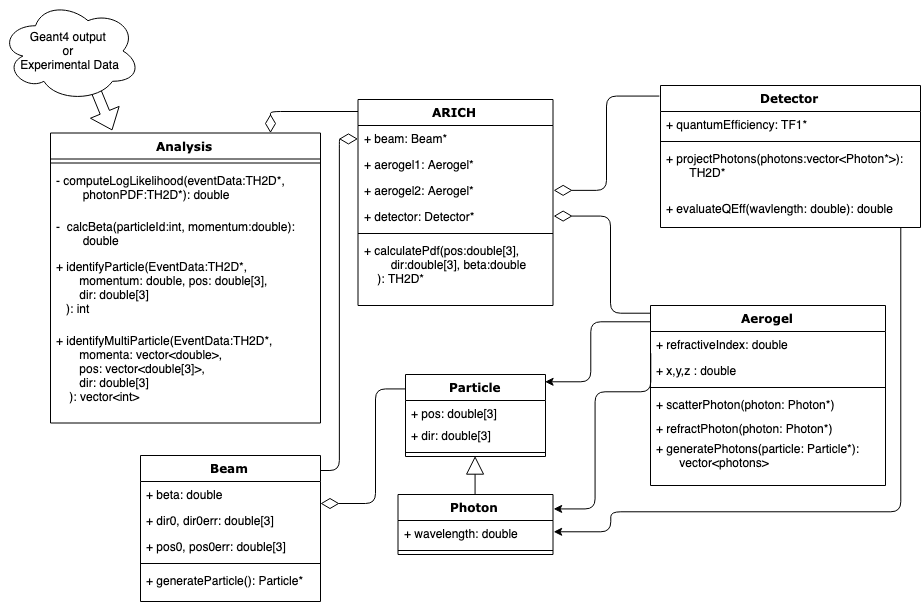
\includegraphics{./figs/uml.png}}
\caption[UML diagram outlining the most important classes and methods used in the simulation and analysis ]{UML diagram outlining the most important classes and methods used in the simulation and analysis. }
\label{fig:uml}

\end{sidewaysfigure}





\backmatter
%    7. Index
% See the makeindex package: the following page provides a quick overview
% <http://www.image.ufl.edu/help/latex/latex_indexes.shtml>


\end{document}
